\PassOptionsToPackage{unicode=true}{hyperref} % options for packages loaded elsewhere
\PassOptionsToPackage{hyphens}{url}
%
\documentclass[10pt,xcolor=table,color={dvipsnames,usenames},ignorenonframetext,usepdftitle=false,french]{beamer}
\setbeamertemplate{caption}[numbered]
\setbeamertemplate{caption label separator}{: }
\setbeamercolor{caption name}{fg=normal text.fg}
\beamertemplatenavigationsymbolsempty
\usepackage{caption}
\captionsetup{skip=0pt,belowskip=0pt}
%\setlength\abovecaptionskip{-15pt}
\usepackage{lmodern}
\usepackage{amssymb,amsmath,mathtools,multirow}
\usepackage{float,hhline}
\usepackage{tikz}
\usepackage[tikz]{bclogo}
\usepackage{mathtools}
\usepackage{ifxetex,ifluatex}
\usepackage{fixltx2e} % provides \textsubscript
\ifnum 0\ifxetex 1\fi\ifluatex 1\fi=0 % if pdftex
  \usepackage[T1]{fontenc}
  \usepackage[utf8]{inputenc}
  \usepackage{textcomp} % provides euro and other symbols
\else % if luatex or xelatex
  \usepackage{unicode-math}
  \defaultfontfeatures{Ligatures=TeX,Scale=MatchLowercase}
\fi
\usetheme[coding=utf8,language=english,
,titlepagelogo=img/SACElogo.jpg
]{TorinoTh}
% use upquote if available, for straight quotes in verbatim environments
\IfFileExists{upquote.sty}{\usepackage{upquote}}{}
% use microtype if available
\IfFileExists{microtype.sty}{%
\usepackage[]{microtype}
\UseMicrotypeSet[protrusion]{basicmath} % disable protrusion for tt fonts
}{}
\IfFileExists{parskip.sty}{%
\usepackage{parskip}
}{% else
\setlength{\parindent}{0pt}
\setlength{\parskip}{6pt plus 2pt minus 1pt}
}
\usepackage{hyperref}
\hypersetup{
            pdftitle={De la conception d'un package à RJDemetra et au-delà},
            pdfauthor={Alain Quartier-la-Tente et Anna Michalek},
            pdfborder={0 0 0},
            breaklinks=true}
\urlstyle{same}  % don't use monospace font for urls
\newif\ifbibliography
\usepackage{color}
\usepackage{fancyvrb}
\newcommand{\VerbBar}{|}
\newcommand{\VERB}{\Verb[commandchars=\\\{\}]}
\DefineVerbatimEnvironment{Highlighting}{Verbatim}{commandchars=\\\{\}}
% Add ',fontsize=\small' for more characters per line
\usepackage{framed}
\definecolor{shadecolor}{RGB}{248,248,248}
\newenvironment{Shaded}{\begin{snugshade}}{\end{snugshade}}
\newcommand{\AlertTok}[1]{\textcolor[rgb]{0.94,0.16,0.16}{#1}}
\newcommand{\AnnotationTok}[1]{\textcolor[rgb]{0.56,0.35,0.01}{\textbf{\textit{#1}}}}
\newcommand{\AttributeTok}[1]{\textcolor[rgb]{0.77,0.63,0.00}{#1}}
\newcommand{\BaseNTok}[1]{\textcolor[rgb]{0.00,0.00,0.81}{#1}}
\newcommand{\BuiltInTok}[1]{#1}
\newcommand{\CharTok}[1]{\textcolor[rgb]{0.31,0.60,0.02}{#1}}
\newcommand{\CommentTok}[1]{\textcolor[rgb]{0.56,0.35,0.01}{\textit{#1}}}
\newcommand{\CommentVarTok}[1]{\textcolor[rgb]{0.56,0.35,0.01}{\textbf{\textit{#1}}}}
\newcommand{\ConstantTok}[1]{\textcolor[rgb]{0.00,0.00,0.00}{#1}}
\newcommand{\ControlFlowTok}[1]{\textcolor[rgb]{0.13,0.29,0.53}{\textbf{#1}}}
\newcommand{\DataTypeTok}[1]{\textcolor[rgb]{0.13,0.29,0.53}{#1}}
\newcommand{\DecValTok}[1]{\textcolor[rgb]{0.00,0.00,0.81}{#1}}
\newcommand{\DocumentationTok}[1]{\textcolor[rgb]{0.56,0.35,0.01}{\textbf{\textit{#1}}}}
\newcommand{\ErrorTok}[1]{\textcolor[rgb]{0.64,0.00,0.00}{\textbf{#1}}}
\newcommand{\ExtensionTok}[1]{#1}
\newcommand{\FloatTok}[1]{\textcolor[rgb]{0.00,0.00,0.81}{#1}}
\newcommand{\FunctionTok}[1]{\textcolor[rgb]{0.00,0.00,0.00}{#1}}
\newcommand{\ImportTok}[1]{#1}
\newcommand{\InformationTok}[1]{\textcolor[rgb]{0.56,0.35,0.01}{\textbf{\textit{#1}}}}
\newcommand{\KeywordTok}[1]{\textcolor[rgb]{0.13,0.29,0.53}{\textbf{#1}}}
\newcommand{\NormalTok}[1]{#1}
\newcommand{\OperatorTok}[1]{\textcolor[rgb]{0.81,0.36,0.00}{\textbf{#1}}}
\newcommand{\OtherTok}[1]{\textcolor[rgb]{0.56,0.35,0.01}{#1}}
\newcommand{\PreprocessorTok}[1]{\textcolor[rgb]{0.56,0.35,0.01}{\textit{#1}}}
\newcommand{\RegionMarkerTok}[1]{#1}
\newcommand{\SpecialCharTok}[1]{\textcolor[rgb]{0.00,0.00,0.00}{#1}}
\newcommand{\SpecialStringTok}[1]{\textcolor[rgb]{0.31,0.60,0.02}{#1}}
\newcommand{\StringTok}[1]{\textcolor[rgb]{0.31,0.60,0.02}{#1}}
\newcommand{\VariableTok}[1]{\textcolor[rgb]{0.00,0.00,0.00}{#1}}
\newcommand{\VerbatimStringTok}[1]{\textcolor[rgb]{0.31,0.60,0.02}{#1}}
\newcommand{\WarningTok}[1]{\textcolor[rgb]{0.56,0.35,0.01}{\textbf{\textit{#1}}}}
\usepackage{graphicx,grffile}
\makeatletter
\def\maxwidth{\ifdim\Gin@nat@width>\linewidth\linewidth\else\Gin@nat@width\fi}
\def\maxheight{\ifdim\Gin@nat@height>\textheight\textheight\else\Gin@nat@height\fi}
\makeatother
% Scale images if necessary, so that they will not overflow the page
% margins by default, and it is still possible to overwrite the defaults
% using explicit options in \includegraphics[width, height, ...]{}
\setkeys{Gin}{width=\maxwidth,height=\maxheight,keepaspectratio}
% Prevent slide breaks in the middle of a paragraph:
\widowpenalties 1 10000
\raggedbottom
\AtBeginPart{
  \let\insertpartnumber\relax
  \let\partname\relax
  \frame{\partpage}
}
\AtBeginSection{
  \ifbibliography
  \else
    \begin{frame}{Sommaire}
    \tableofcontents[currentsection, hideothersubsections]
    \end{frame}
  \fi
}
\setlength{\emergencystretch}{3em}  % prevent overfull lines
\providecommand{\tightlist}{%
  %\setlength{\itemsep}{0pt}
  \setlength{\parskip}{0pt}
  }
\setcounter{secnumdepth}{0}

% set default figure placement to htbp
\makeatletter
\def\fps@figure{htbp}
\makeatother

\usepackage{wrapfig}
\usepackage{booktabs}
\usepackage{longtable}
\usepackage{array}
\usepackage{multirow}
\usepackage[table]{xcolor}
\usepackage{wrapfig}
\usepackage{float}
\usepackage{colortbl}
\usepackage{pdflscape}
\usepackage{tabu}
\usepackage{threeparttable}
\usepackage{threeparttablex}
\usepackage[normalem]{ulem}
\usepackage{makecell}
\usepackage{animate}
\usepackage{fontawesome5}

\title{De la conception d'un package à RJDemetra et au-delà}
\ateneo{Séminaire interne DMS, 4 avril 2019}
\author{Alain Quartier-la-Tente et Anna Michalek}
\date{}


\setrellabel{}

\setcandidatelabel{}

\rel{}
\division{Insee, Seasonal Adjustment Centre of Excellence (AQLT) and European
Central Bank (AM)}

\departement{\href{mailto:alain.quartier-la-tente@insee.fr}{\nolinkurl{alain.quartier-la-tente@insee.fr}}}
\makeatletter
\let\@@magyar@captionfix\relax
\makeatother

\DeclareMathOperator{\Cov}{Cov}
\newcommand{\E}[1]{\mathbb{E}\left[ #1 \right]}
\newcommand{\V}[1]{\mathbb{V}\left[ #1 \right]}
\newcommand{\cov}[2]{\Cov\left( #1\,,\,#2 \right)}

\begin{document}
\begin{frame}[plain,noframenumbering]
\titlepage
\end{frame}

\hypertarget{introduction}{%
\section{Introduction}\label{introduction}}

\begin{frame}{RJDemetra et JDemetra+ \bcquestion}
\protect\hypertarget{rjdemetra-et-jdemetra}{}


\includegraphics[width=2cm]{img/jdemetra+.png} JDemetra+ (JD+) :
logiciel de désaisonnalisation,
\href{https://ec.europa.eu/eurostat/cros/system/files/Jdemetra_\%20release.pdf}{officiellement
recommandé} par Eurostat et la BCE, où sont implémentés TRAMO/SEATS+ et
X-13ARIMA-SEATS

\bigskip

\(\rightarrow\) RJDemetra est une interface \large\faRProject{}
\normalsize à JDemetra+ basée sur les librairies \large\faJava{}
\normalsize de JD+

\pause

Objectif : avoir un package complet autour de JD+ dans un langage de
script (ici \faRProject) accessible à tous pour :

\begin{itemize}
\item
  tester sans développer une interface graphique
\item
  utiliser ce qui est déjà disponible en R
\item
  faire des nouveaux développements (dashboards, direct vs indirect)
\end{itemize}

\end{frame}

\hypertarget{creation-dun-package-java}{%
\section{Création d'un package Java}\label{creation-dun-package-java}}

\hypertarget{creation-dun-package}{%
\subsection{Création d'un package}\label{creation-dun-package}}

\begin{frame}{6 idées reçues sur la création d'un package}
\protect\hypertarget{idees-recues-sur-la-creation-dun-package}{}

\begin{enumerate}
\item
  Réaliser un package est un truc d'initié
\item
  Un package est à destination du CRAN
\item
  Un package sert à partager son code avec d'autres personnes
\item
  Je n'ai que très peu de fonctions, inutile d'en faire un package
\item
  Cela prend du temps
\end{enumerate}

\(\rightarrow\) Beaucoup de documentation en ligne en \bcdfrance

Exemple : ``Fabriquer un package R en moins de 6 minutes''
\url{https://r2018-rennes.sciencesconf.org/205552}

\(\rightarrow\) Pour aller plus loin : ``R packages''
\url{http://r-pkgs.had.co.nz/}

\(\rightarrow\) utilisation de RStudio

\end{frame}

\begin{frame}{Faire son premier package (1/5)}
\protect\hypertarget{faire-son-premier-package-15}{}

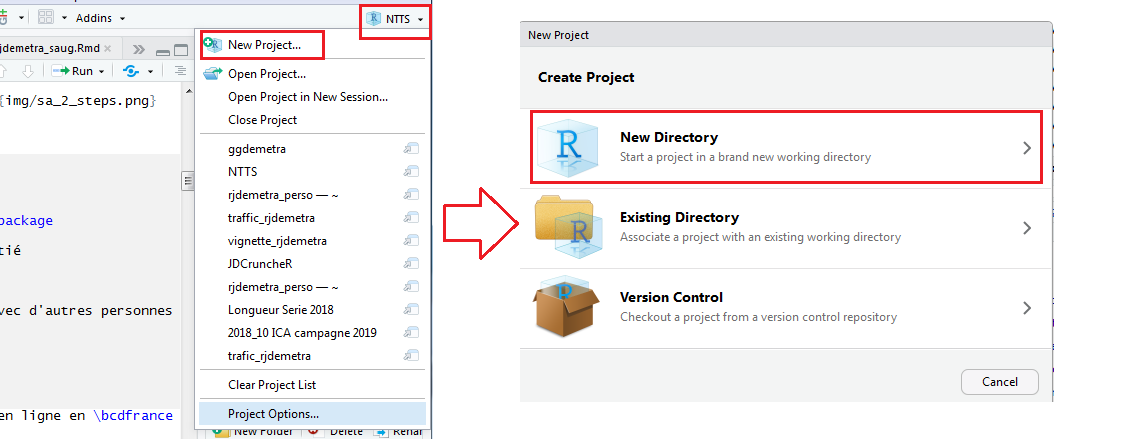
\includegraphics{img/package/new_project00.png}

\end{frame}

\begin{frame}{Faire son premier package (2/5)}
\protect\hypertarget{faire-son-premier-package-25}{}

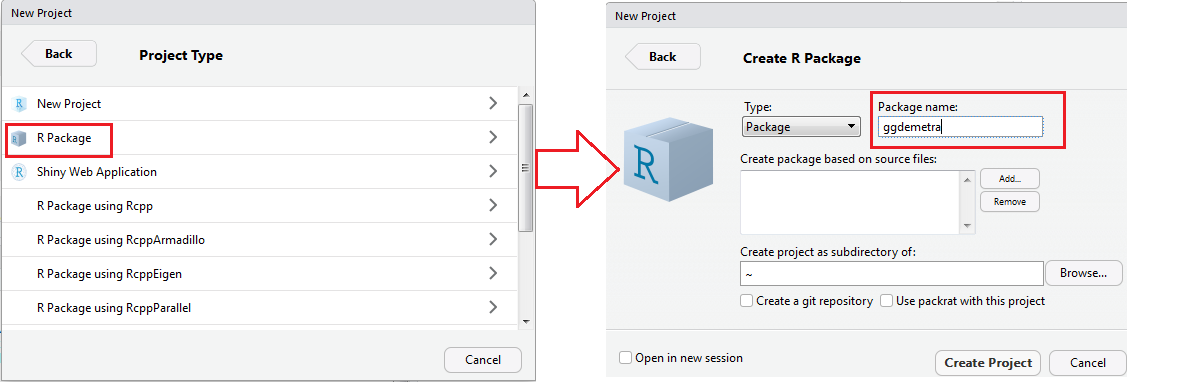
\includegraphics{img/package/new_project01.png}

\end{frame}

\begin{frame}{Faire son premier package (3/5)}
\protect\hypertarget{faire-son-premier-package-35}{}

Plusieurs dossiers sont créés :

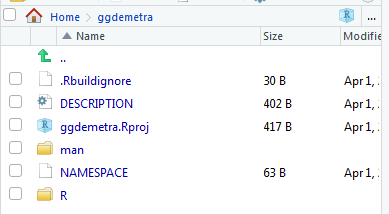
\includegraphics[width = 0.2\textwidth]{img/package/new_project03.png}

Les plus importants :

\begin{itemize}
\tightlist
\item
  dossier R : programmes R
\item
  DESCRIPTION : description du package
\item
  NAMESPACE et man : seront générés automatiquement
\end{itemize}

\end{frame}

\begin{frame}{Faire son premier package (4/5)}
\protect\hypertarget{faire-son-premier-package-45}{}

Exemple du DESCRIPTION

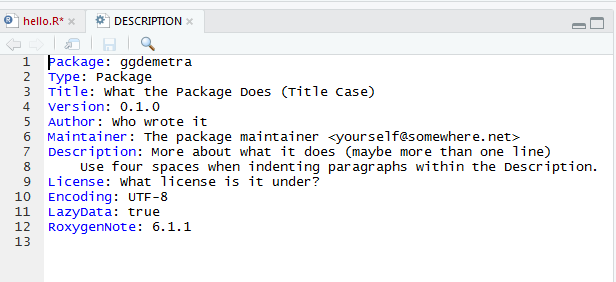
\includegraphics{img/package/new_project04.png}

\end{frame}

\begin{frame}{Faire son premier package (5/5)}
\protect\hypertarget{faire-son-premier-package-55}{}

Programme par défaut :

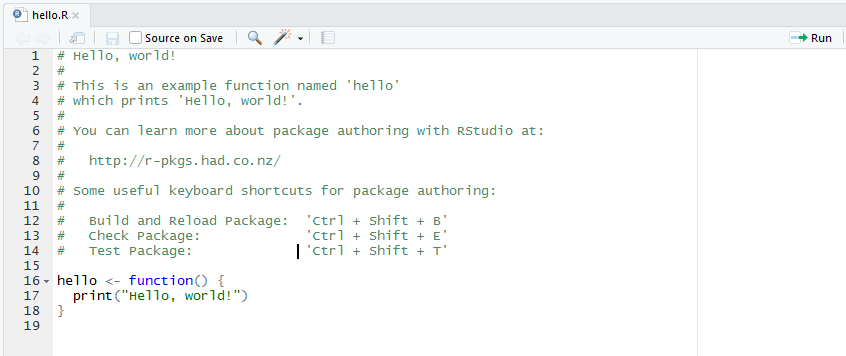
\includegraphics{img/package/new_project02.png}

\begin{itemize}
\item
  Check : vérifier s'il n'y a pas d'erreur d'exécution ou de codage
  `Ctrl + Shift + E'
\item
  Build and Reload : installer le package
\end{itemize}

\end{frame}

\begin{frame}{Documentation avec roxygen2 (1/3)}
\protect\hypertarget{documentation-avec-roxygen2-13}{}

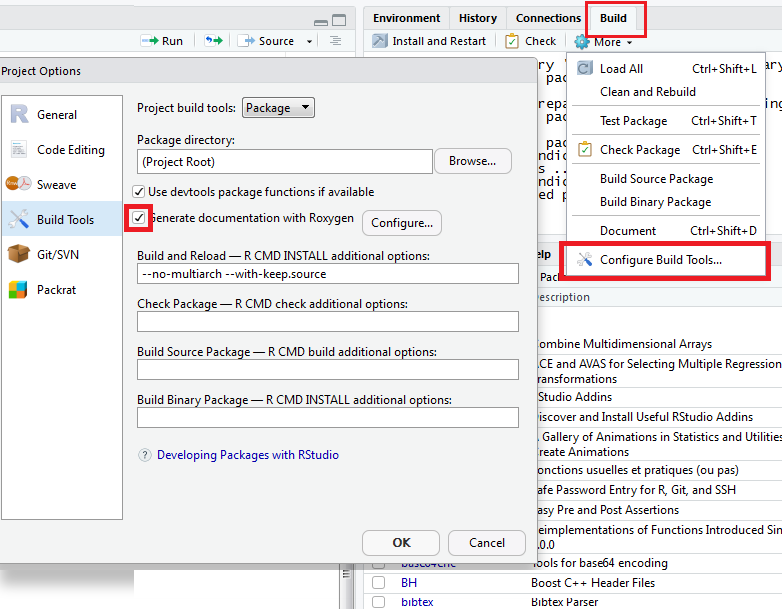
\includegraphics{img/package/fonction01.png}

\end{frame}

\begin{frame}{Documentation avec roxygen2 (2/3)}
\protect\hypertarget{documentation-avec-roxygen2-23}{}

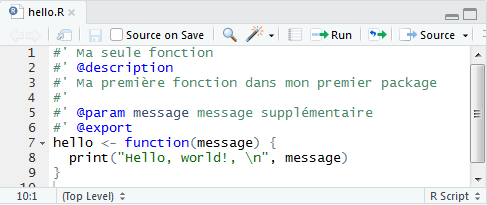
\includegraphics[width=0.9\textwidth]{img/package/fonction02.png}

\end{frame}

\begin{frame}{Documentation avec roxygen2 (3/3)}
\protect\hypertarget{documentation-avec-roxygen2-33}{}

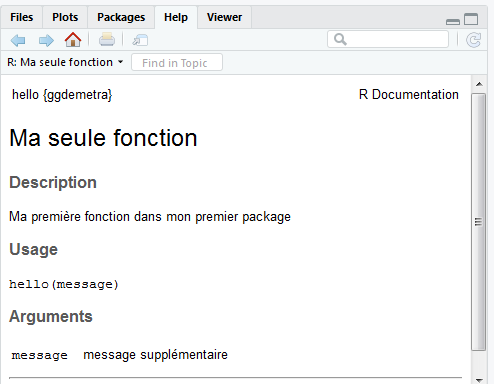
\includegraphics[width=0.9\textwidth]{img/package/fonction03.png}

\end{frame}

\hypertarget{lien-avec-java}{%
\subsection{Lien avec Java}\label{lien-avec-java}}

\begin{frame}[fragile]{rJava}
\protect\hypertarget{rjava}{}

Dans une session R :

\begin{Shaded}
\begin{Highlighting}[]
\KeywordTok{library}\NormalTok{(}\StringTok{"rJava"}\NormalTok{)}
\KeywordTok{.jinit}\NormalTok{()}
\KeywordTok{.jaddClassPath}\NormalTok{(}\StringTok{"./inst/java/demetra-tstoolkit-2.2.2.jar"}\NormalTok{)}
\KeywordTok{.jaddClassPath}\NormalTok{(}\StringTok{"./inst/java/jdr-2.2.2.jar"}\NormalTok{)}
\end{Highlighting}
\end{Shaded}

\pause

Dans un package : librairies \faJava{} sous \texttt{/inst/java}

\begin{Shaded}
\begin{Highlighting}[]
\NormalTok{.onLoad <-}\StringTok{ }\ControlFlowTok{function}\NormalTok{(libname, pkgname)\{}
  \KeywordTok{.jpackage}\NormalTok{(pkgname, }\DataTypeTok{lib.loc =}\NormalTok{ libname)}
\NormalTok{\}}
\end{Highlighting}
\end{Shaded}

\pause

Deux fonctions à retenir :

\begin{enumerate}
\item
  \texttt{.jcall()} : appeler une méthode
\item
  \texttt{.jnew()} : créer un nouveau objet Java
\end{enumerate}

\end{frame}

\begin{frame}[fragile]{Un exemple}
\protect\hypertarget{un-exemple}{}

\begin{Shaded}
\begin{Highlighting}[]
\KeywordTok{library}\NormalTok{(rJava)}
\KeywordTok{library}\NormalTok{(RJDemetra)}
\NormalTok{jrspec <-}\StringTok{ }\KeywordTok{.jcall}\NormalTok{(}\StringTok{"jdr/spec/tramoseats/TramoSeatsSpec"}\NormalTok{,}
                 \StringTok{"Ljdr/spec/tramoseats/TramoSeatsSpec;"}\NormalTok{,}
                 \StringTok{"of"}\NormalTok{, }\StringTok{"RSA0"}\NormalTok{)}
\NormalTok{jspec <-}\StringTok{ }\KeywordTok{.jcall}\NormalTok{(jrspec,}
                \StringTok{"Lec/satoolkit/tramoseats/TramoSeatsSpecification;"}\NormalTok{,}
                \StringTok{"getCore"}\NormalTok{)}\CommentTok{# ou : jspec <- jrspec$getCore()}
\NormalTok{jdictionary <-}\StringTok{ }\KeywordTok{.jnew}\NormalTok{(}\StringTok{"jdr/spec/ts/Utility$Dictionary"}\NormalTok{)}
\NormalTok{jrslt <-}\StringTok{ }\KeywordTok{.jcall}\NormalTok{(}\StringTok{"ec/tstoolkit/jdr/sa/Processor"}\NormalTok{,}
                \StringTok{"Lec/tstoolkit/jdr/sa/TramoSeatsResults;"}\NormalTok{,}
                \StringTok{"tramoseats"}\NormalTok{,}
\NormalTok{                RJDemetra}\OperatorTok{:::}\KeywordTok{ts_r2jd}\NormalTok{(ipi_c_eu[,}\StringTok{"FR"}\NormalTok{]),}
\NormalTok{                jspec, jdictionary)}
\NormalTok{jrslt}
\end{Highlighting}
\end{Shaded}

\begin{verbatim}
## [1] "Java-Object{TramoSeatsResults(results=ec.tstoolkit.algorithm.CompositeResults@2bea5ab4, diagnostics=ec.tstoolkit.jdr.sa.SaDiagnostics@3d8314f0)}"
\end{verbatim}

\end{frame}

\hypertarget{tests-et-diffusion}{%
\subsection{Tests et diffusion}\label{tests-et-diffusion}}

\begin{frame}[fragile]{Tester son package}
\protect\hypertarget{tester-son-package}{}

\begin{itemize}
\tightlist
\item
  R CMD CHECK : tests sur sa machine
\end{itemize}

\pause

\begin{itemize}
\tightlist
\item
  \texttt{rhub} pour lancer R CMD CHECK sur différentes plateformes
  (debian, linux, macos\ldots{}) : \texttt{rhub::check\_for\_cran()}\\
  \faGithub{} \url{https://r-hub.github.io/rhub/index.html}
\end{itemize}

\pause

\begin{itemize}
\tightlist
\item
  Intégration continue avec GitHub \(\rightarrow\) Ex avec TRAVIS CI, il
  suffit de créer un fichier \texttt{.travis.yml} dans son package et de
  configurer GitHub
\end{itemize}

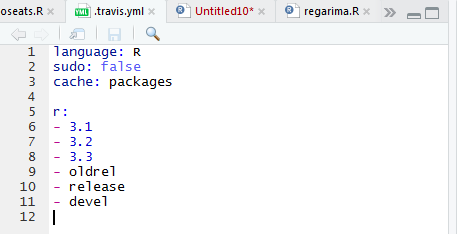
\includegraphics{img/package/travis.png}

\end{frame}

\begin{frame}[fragile]{Site web automatique}
\protect\hypertarget{site-web-automatique}{}

\texttt{pkgdown} permet de générer un site web, à partir de la
documentation, qui peut être hébergé sur GitHub :

\begin{itemize}
\item
  Plus lisible
\item
  Accessible sans avoir à ouvrir R
\item
  Résultats des exemples
\end{itemize}

\begin{Shaded}
\begin{Highlighting}[]
\NormalTok{pkgdown}\OperatorTok{::}\KeywordTok{build_site}\NormalTok{()}
\end{Highlighting}
\end{Shaded}

Exemple :

\url{https://jdemetra.github.io/rjdemetra/}

\end{frame}

\begin{frame}{Diffusion d'un package}
\protect\hypertarget{diffusion-dun-package}{}

Grande communité \large\faRProject{} \normalsize sur Twitter\\
\(\rightarrow\)
\href{https://twitter.com/JDemetraPlus}{\faTwitter{} @JdemetraPlus}\\
\(\rightarrow\) rôle de l'Insee ?

De nombreuses conférences autour de R en France et en Europe : RLadies,
RAddicts, RUSS, satRdays, useR!, Rencontres R, eRum, uRos\ldots{}

Impression de ``goodies'' :

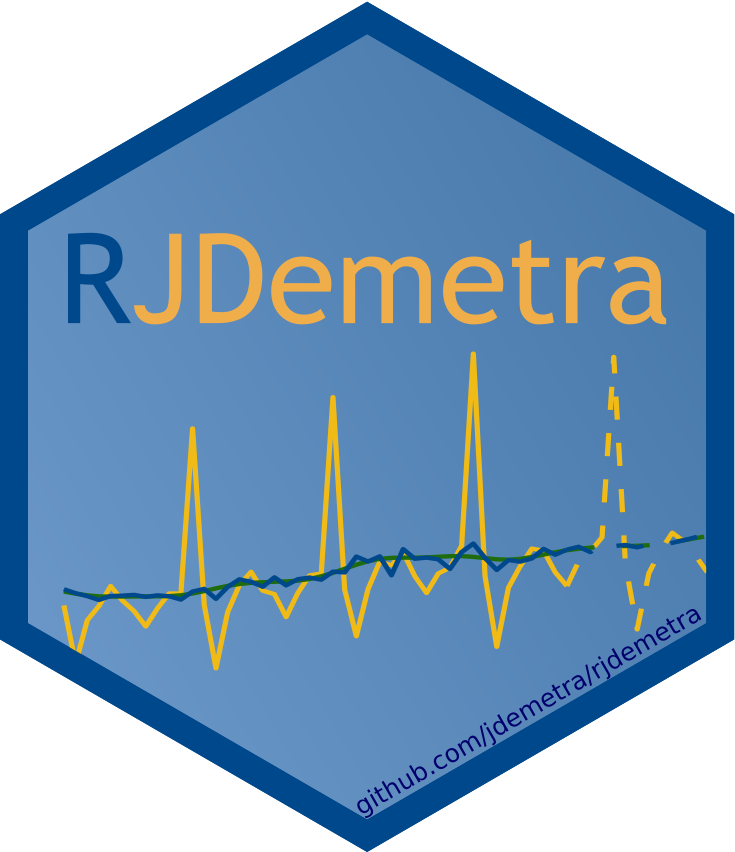
\includegraphics[width=3cm]{img/rjdemetra_logo.png}

\includegraphics[width=3cm]{img/jdemetra+.png}

\end{frame}

\hypertarget{rjdemetra}{%
\section{RJDemetra}\label{rjdemetra}}

\begin{frame}{Les deux étapes de la désaisonnalisation}
\protect\hypertarget{les-deux-etapes-de-la-desaisonnalisation}{}

\vspace{-0.15cm}

\begin{enumerate}
\item
  Pre-ajustement de certains effets déterministes par un modèle RegARIMA
\item
  Décomposition: pour extraire la composante saisonnière
\end{enumerate}

\centering

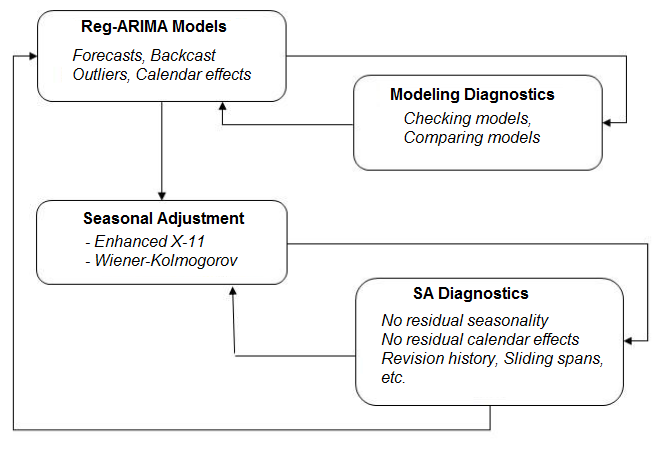
\includegraphics[height=0.75\textheight]{img/sa_2_steps.png}

\end{frame}

\hypertarget{current-status}{%
\subsection{Current status}\label{current-status}}

\begin{frame}{Current status}
\protect\hypertarget{current-status-1}{}

\begin{itemize}
\tightlist
\item
  RegARIMA, TRAMO-SEATS et X-13-ARIMA :

  \begin{itemize}
  \tightlist
  \item
    spécifications prédéfinies et personnalisées
  \item
    classes S3 avec des méthodes plot, summary, print
  \end{itemize}
\end{itemize}

\medskip

\begin{itemize}
\tightlist
\item
  Manipulation de workspaces JD+ :

  \begin{itemize}
  \tightlist
  \item
    Import de workspaces to avec le modèle CVS
  \item
    Export des modèles R créé par RJDemetra
  \end{itemize}
\end{itemize}

\medskip

\begin{itemize}
\tightlist
\item
  Contient une base de données : les IPI dans l'industrie manufacturière
  dans l'UE
\end{itemize}

\end{frame}

\hypertarget{regarima-exemples}{%
\subsection{RegARIMA : exemples}\label{regarima-exemples}}

\begin{frame}[fragile]{RegARIMA : exemples (1/4)}
\protect\hypertarget{regarima-exemples-14}{}

\begin{Shaded}
\begin{Highlighting}[]
\KeywordTok{library}\NormalTok{(RJDemetra)}
\NormalTok{ipi_fr <-}\StringTok{ }\NormalTok{ipi_c_eu[,}\StringTok{"FR"}\NormalTok{]}
\NormalTok{regarima_model <-}\StringTok{ }\KeywordTok{regarima_def_x13}\NormalTok{(ipi_fr, }\DataTypeTok{spec =} \StringTok{"RG4c"}\NormalTok{)}
\NormalTok{regarima_model}
\end{Highlighting}
\end{Shaded}

\begin{verbatim}
## y = regression model + arima (2, 1, 1, 0, 1, 1)
## Log-transformation: no
## Coefficients:
##           Estimate Std. Error
## Phi(1)      0.3358      0.171
## Phi(2)      0.2060      0.096
## Theta(1)   -0.2450      0.173
## BTheta(1)  -0.5112      0.050
## 
##              Estimate Std. Error
## Easter [1]     -1.133      0.337
## LS (11-2008)   -8.000      1.283
## LS (1-2009)    -7.551      1.283
## LS (5-2008)    -5.069      1.234
## 
## 
## Residual standard error: 1.696 on 323 degrees of freedom
## Log likelihood =  -631, aic =  1280 aicc =  1281, bic(corrected for length) =   1.2
\end{verbatim}

\end{frame}

\begin{frame}[fragile]{RegARIMA : exemples (2/4)}
\protect\hypertarget{regarima-exemples-24}{}

\footnotesize

\begin{Shaded}
\begin{Highlighting}[]
\KeywordTok{summary}\NormalTok{(regarima_model)}
\end{Highlighting}
\end{Shaded}

\begin{verbatim}
## y = regression model + arima (2, 1, 1, 0, 1, 1)
## 
## Model: RegARIMA - X13
## Estimation span: from 1-1990 to 12-2017
## Log-transformation: no
## Regression model: no mean, no trading days effect, no leap year effect, Easter effect, outliers(3)
## 
## Coefficients:
## ARIMA: 
##           Estimate Std. Error  T-stat Pr(>|t|)    
## Phi(1)     0.33579    0.17106   1.963   0.0505 .  
## Phi(2)     0.20600    0.09643   2.136   0.0334 *  
## Theta(1)  -0.24498    0.17272  -1.418   0.1571    
## BTheta(1) -0.51123    0.05004 -10.216   <2e-16 ***
## ---
## Signif. codes:  0 '***' 0.001 '**' 0.01 '*' 0.05 '.' 0.1 ' ' 1
## 
## Regression model: 
##              Estimate Std. Error T-stat Pr(>|t|)    
## Easter [1]    -1.1332     0.3373 -3.359 0.000875 ***
## LS (11-2008)  -7.9997     1.2831 -6.235 1.42e-09 ***
## LS (1-2009)   -7.5508     1.2833 -5.884 1.00e-08 ***
## LS (5-2008)   -5.0692     1.2341 -4.108 5.07e-05 ***
## ---
## Signif. codes:  0 '***' 0.001 '**' 0.01 '*' 0.05 '.' 0.1 ' ' 1
## 
## 
## Residual standard error: 1.696 on 9 degrees of freedom
## Log likelihood =  -631, aic =  1280, aicc =  1281, bic(corrected for length) =   1.2
\end{verbatim}

\end{frame}

\begin{frame}[fragile]{RegARIMA : exemples (3/4)}
\protect\hypertarget{regarima-exemples-34}{}

\begin{Shaded}
\begin{Highlighting}[]
\KeywordTok{layout}\NormalTok{(}\KeywordTok{matrix}\NormalTok{(}\DecValTok{1}\OperatorTok{:}\DecValTok{6}\NormalTok{, }\DecValTok{3}\NormalTok{, }\DecValTok{2}\NormalTok{));}\KeywordTok{plot}\NormalTok{(regarima_model, }\DataTypeTok{ask =} \OtherTok{FALSE}\NormalTok{)}
\end{Highlighting}
\end{Shaded}

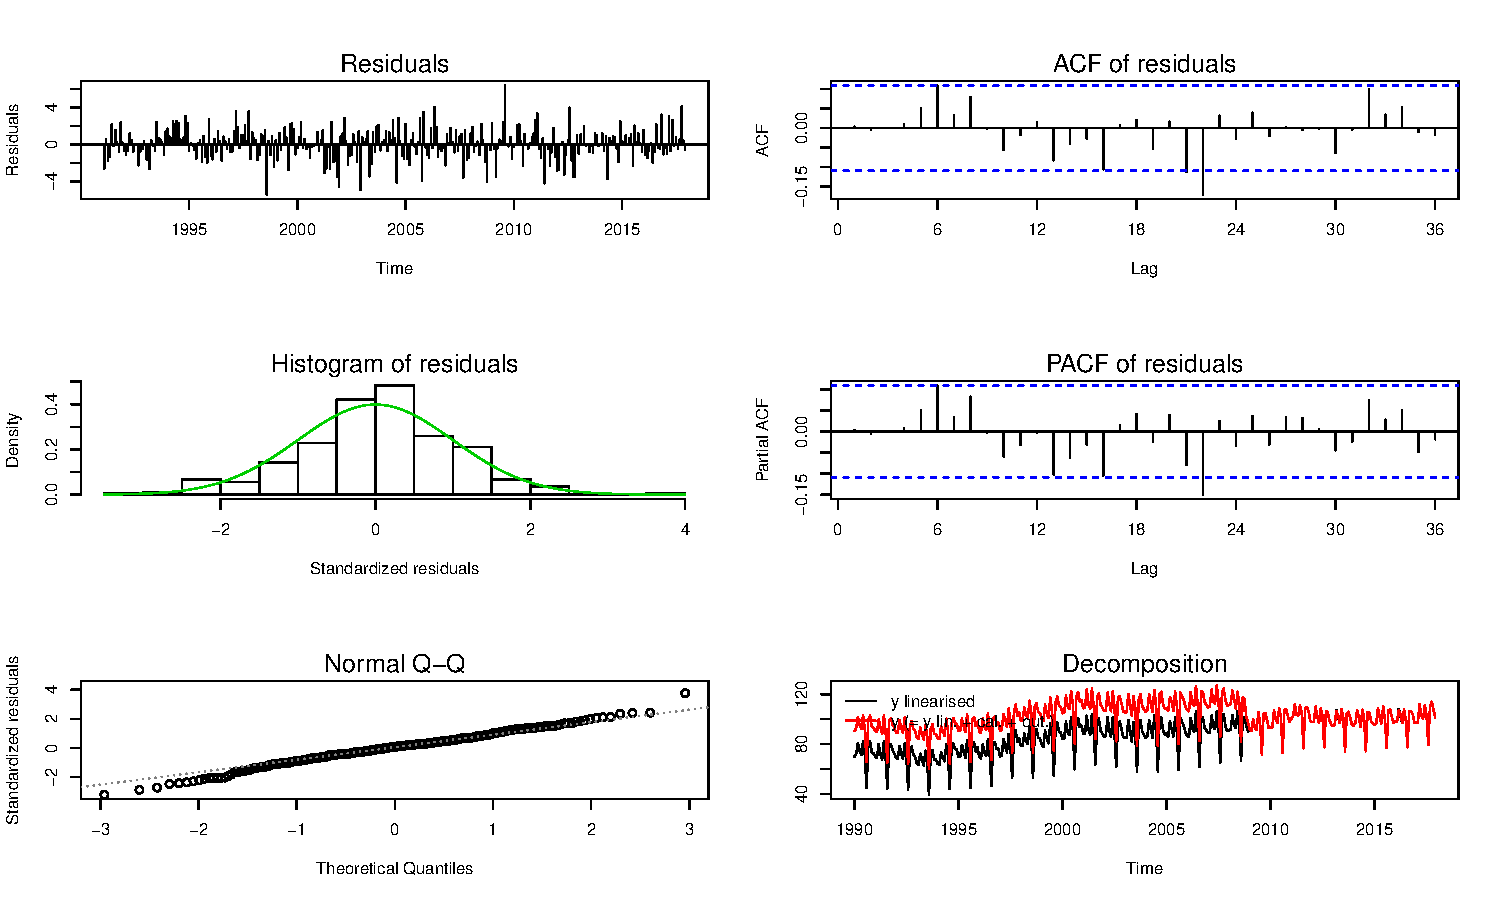
\includegraphics{img/markdown-unnamed-chunk-8-1.pdf}

\end{frame}

\begin{frame}[fragile]{RegARIMA : exemples (4/4)}
\protect\hypertarget{regarima-exemples-44}{}

\begin{Shaded}
\begin{Highlighting}[]
\KeywordTok{plot}\NormalTok{(regarima_model, }\DataTypeTok{which =} \DecValTok{7}\NormalTok{)}
\end{Highlighting}
\end{Shaded}

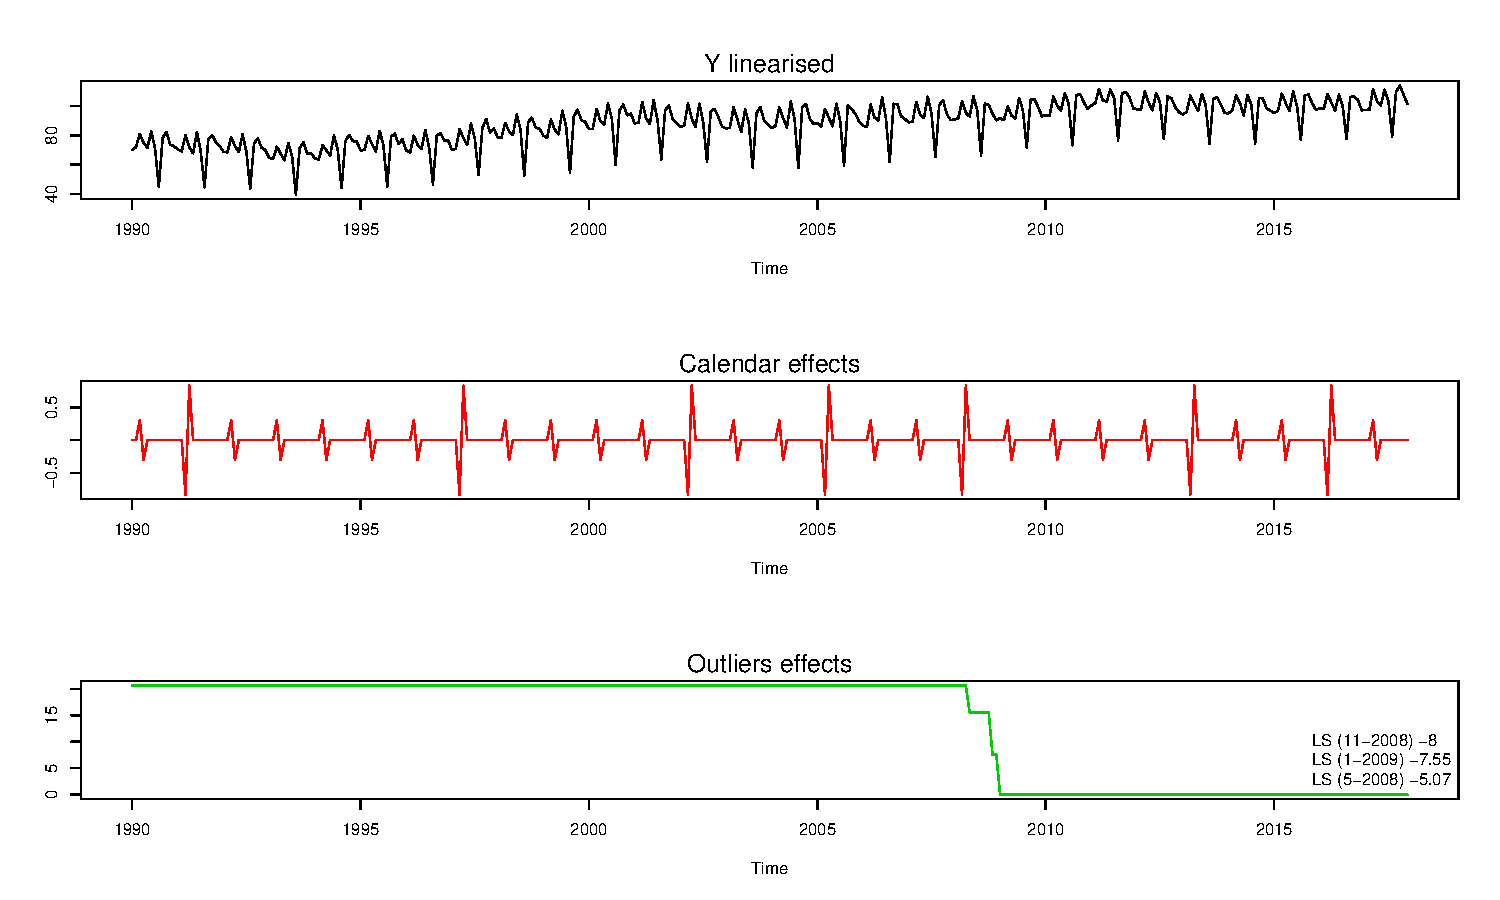
\includegraphics{img/markdown-unnamed-chunk-10-1.pdf}

\end{frame}

\hypertarget{cvs-cjo-exemples}{%
\subsection{CVS-CJO : exemples}\label{cvs-cjo-exemples}}

\begin{frame}[fragile]{CVS-CJO : exemples (1/8)}
\protect\hypertarget{cvs-cjo-exemples-18}{}

Un object \texttt{SA} est une \texttt{list()} de 5 éléments:

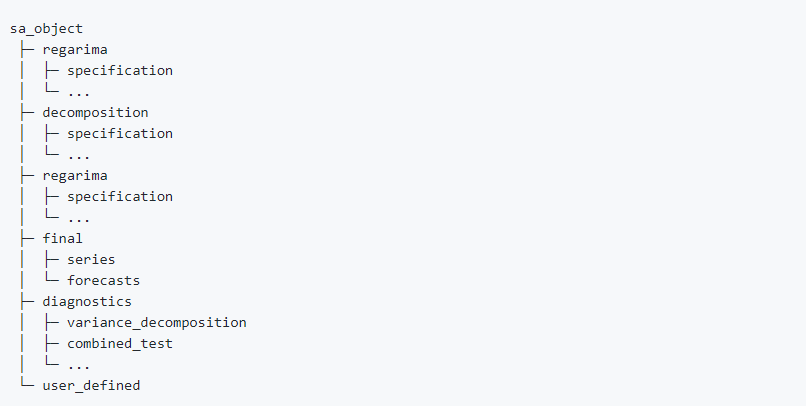
\includegraphics{img/sa_obj_struct.png}

\end{frame}

\begin{frame}[fragile]{CVS-CJO : exemples (2/8)}
\protect\hypertarget{cvs-cjo-exemples-28}{}

Possibilité de définir ses propres spécifications comme sous JD+ ou
d'utiliser les spécifications prédéfinies:

\footnotesize

\begin{Shaded}
\begin{Highlighting}[]
\NormalTok{x13_usr_spec <-}\StringTok{ }\KeywordTok{x13_spec_def}\NormalTok{(}\DataTypeTok{spec =} \KeywordTok{c}\NormalTok{(}\StringTok{"RSA5c"}\NormalTok{),}
                             \DataTypeTok{usrdef.outliersEnabled =} \OtherTok{TRUE}\NormalTok{,}
                             \DataTypeTok{usrdef.outliersType =} \KeywordTok{c}\NormalTok{(}\StringTok{"LS"}\NormalTok{, }\StringTok{"AO"}\NormalTok{),}
                             \DataTypeTok{usrdef.outliersDate =} \KeywordTok{c}\NormalTok{(}\StringTok{"2008-10-01"}\NormalTok{,}
                                                     \StringTok{"2002-01-01"}\NormalTok{),}
                             \DataTypeTok{usrdef.outliersCoef =} \KeywordTok{c}\NormalTok{(}\DecValTok{36}\NormalTok{, }\DecValTok{14}\NormalTok{),}
                             \DataTypeTok{transform.function =} \StringTok{"None"}\NormalTok{)}
\NormalTok{x13_mod <-}\StringTok{ }\KeywordTok{x13}\NormalTok{(ipi_fr, x13_usr_spec)}
\NormalTok{ts_mod <-}\StringTok{ }\KeywordTok{tramoseats_def}\NormalTok{(ipi_fr, }\DataTypeTok{spec =} \StringTok{"RSAfull"}\NormalTok{)}
\end{Highlighting}
\end{Shaded}

\end{frame}

\begin{frame}[fragile]{CVS-CJO : exemples (3/8): decomposition}
\protect\hypertarget{cvs-cjo-exemples-38-decomposition}{}

\footnotesize

\begin{Shaded}
\begin{Highlighting}[]
\NormalTok{x13_mod}\OperatorTok{$}\NormalTok{decomposition}
\end{Highlighting}
\end{Shaded}

\begin{verbatim}
##  Monitoring and Quality Assessment Statistics:  
##       M stats
## M(1)    0.055
## M(2)    0.041
## M(3)    0.926
## M(4)    0.621
## M(5)    0.724
## M(6)    0.215
## M(7)    0.074
## M(8)    0.208
## M(9)    0.056
## M(10)   0.158
## M(11)   0.146
## Q       0.297
## Q-M2    0.329
## 
## Final filters: 
## Seasonal filter:  3x5
## Trend filter:  13 terms Henderson moving average
\end{verbatim}

\end{frame}

\begin{frame}[fragile]{CVS-CJO : exemples (4/8): decomposition}
\protect\hypertarget{cvs-cjo-exemples-48-decomposition}{}

\footnotesize

\begin{Shaded}
\begin{Highlighting}[]
\NormalTok{ts_mod}\OperatorTok{$}\NormalTok{decomposition}
\end{Highlighting}
\end{Shaded}

\begin{verbatim}
## Model
## AR :  1 + 0.352498 B + 0.133616 B^2 
## D :  1 - B - B^12 + B^13 
## MA :  1 - 0.186819 B - 0.610856 B^12 + 0.114119 B^13 
## 
## 
## SA
## D :  1 - 2.000000 B + B^2 
## MA :  1 - 1.314459 B + 0.340427 B^2 
## Innovation variance:  0.4669153 
## 
## Trend
## D :  1 - 2.000000 B + B^2 
## MA :  1 + 0.040206 B - 0.959794 B^2 
## Innovation variance:  0.04869563 
## 
## Seasonal
## AR :  1 + 0.352498 B + 0.133616 B^2 
## D :  1 + B + B^2 + B^3 + B^4 + B^5 + B^6 + B^7 + B^8 + B^9 + B^10 + B^11 
## MA :  1 + 0.717848 B + 0.460721 B^2 + 0.310085 B^3 + 0.132447 B^4 - 0.049053 B^5 - 0.216655 B^6 - 0.354556 B^7 - 0.445030 B^8 - 0.469587 B^9 - 0.376625 B^10 - 0.166397 B^11 - 0.410618 B^12 - 0.132580 B^13 
## Innovation variance:  0.1601924 
## 
## Irregular
## Innovation variance:  0.2056884
\end{verbatim}

\end{frame}

\begin{frame}[fragile]{CVS-CJO : exemples (5/8)}
\protect\hypertarget{cvs-cjo-exemples-58}{}

\begin{Shaded}
\begin{Highlighting}[]
\KeywordTok{plot}\NormalTok{(x13_mod}\OperatorTok{$}\NormalTok{decomposition)}
\end{Highlighting}
\end{Shaded}

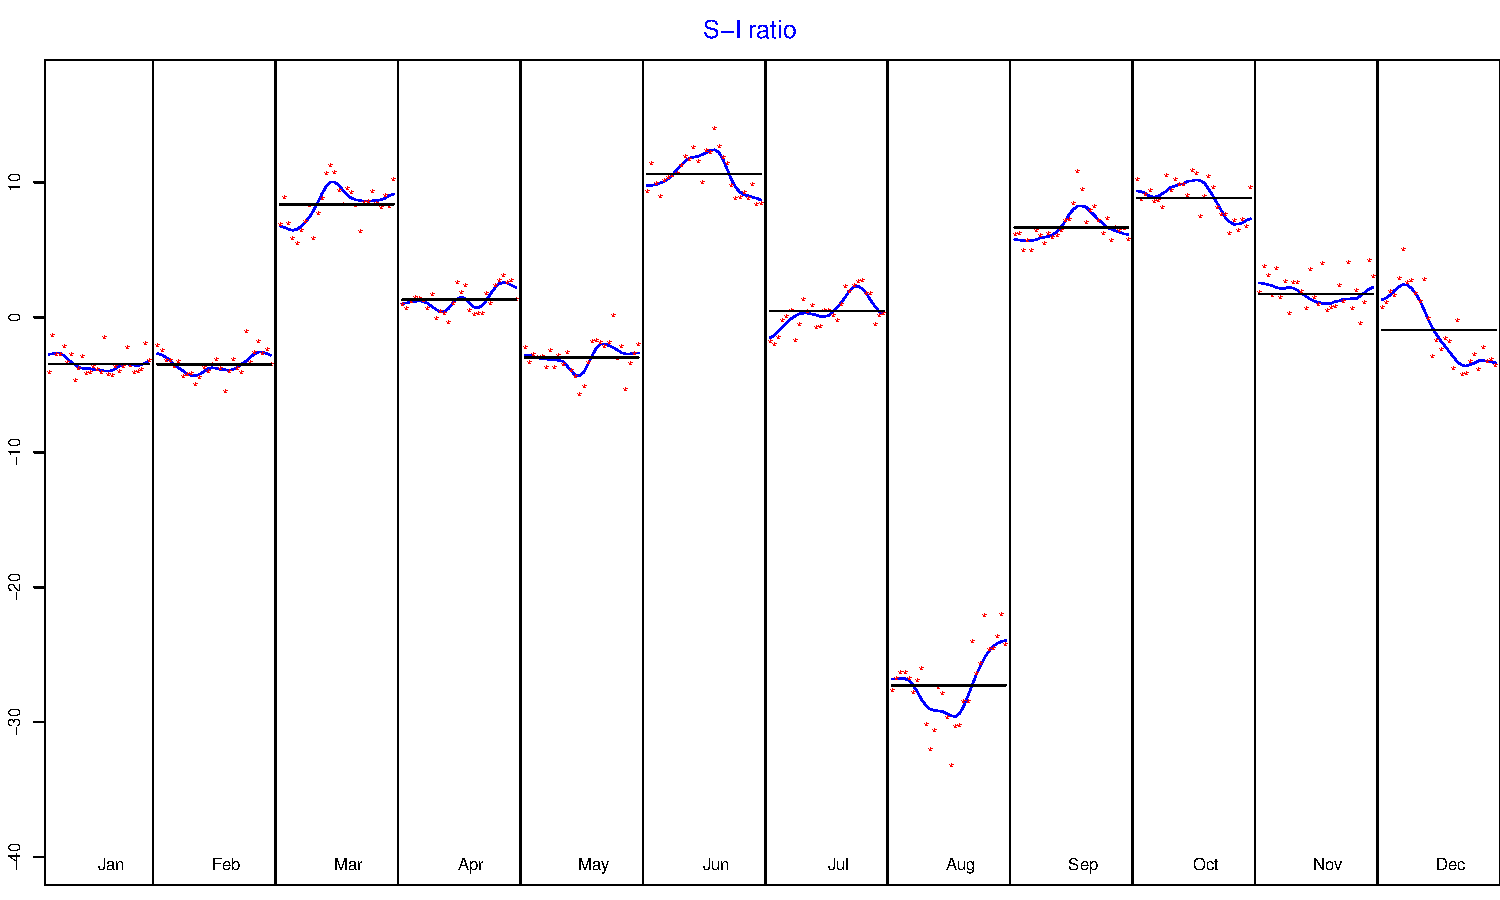
\includegraphics{img/markdown-unnamed-chunk-14-1.pdf}

\end{frame}

\begin{frame}[fragile]{CVS-CJO : exemples (6/8)}
\protect\hypertarget{cvs-cjo-exemples-68}{}

\footnotesize

\begin{Shaded}
\begin{Highlighting}[]
\NormalTok{x13_mod}\OperatorTok{$}\NormalTok{final}
\end{Highlighting}
\end{Shaded}

\begin{verbatim}
## Last observed values
##              y       sa        t           s             i
## Jan 2017  97.4 100.6172 100.6174  -3.2172329 -0.0001992082
## Feb 2017  97.5 100.3127 101.0283  -2.8126932 -0.7155966863
## Mar 2017 112.0 102.5469 101.4894   9.4530696  1.0575376567
## Apr 2017 103.0 101.0897 101.9282   1.9103111 -0.8385432983
## May 2017 100.4 103.0319 102.3136  -2.6318733  0.7182480125
## Jun 2017 111.2 102.4926 102.6921   8.7074293 -0.1994894034
## Jul 2017 103.4 103.1596 103.0816   0.2404277  0.0779236963
## Aug 2017  79.3 103.2483 103.5055 -23.9483256 -0.2572170473
## Sep 2017 109.7 103.5536 103.9555   6.1464361 -0.4019376040
## Oct 2017 114.0 106.6886 104.3955   7.3113786  2.2931579296
## Nov 2017 107.7 105.4631 104.7505   2.2369236  0.7125546908
## Dec 2017 101.4 104.7490 105.0214  -3.3490189 -0.2723590878
## 
## Forecasts:
##                y_f     sa_f      t_f         s_f          i_f
## Jan 2018 101.96630 105.0963 105.1795  -3.1299775 -0.083200162
## Feb 2018 102.23632 105.1464 105.2838  -2.9100563 -0.137428535
## Mar 2018 113.85794 105.5026 105.3966   8.3553336  0.105971540
## Apr 2018 108.47477 105.4896 105.5573   2.9851827 -0.067754048
## May 2018 103.22164 105.7963 105.7844  -2.5746309  0.011859024
## Jun 2018 114.64042 106.0073 106.0629   8.6331483 -0.055612674
## Jul 2018 106.53519 106.3942 106.3666   0.1410119  0.027594337
## Aug 2018  82.77073 106.6890 106.6849 -23.9182264  0.004061745
## Sep 2018 112.79551 106.7018 106.9859   6.0936895 -0.284129714
## Oct 2018 115.13202 107.7516 107.2471   7.3803800  0.504589345
## Nov 2018 109.87965 107.5136 107.4572   2.3660966  0.056314698
## Dec 2018 103.97193 107.3744 107.6093  -3.4024325 -0.234923742
\end{verbatim}

\end{frame}

\begin{frame}[fragile]{CVS-CJO : exemples (7/8)}
\protect\hypertarget{cvs-cjo-exemples-78}{}

\begin{Shaded}
\begin{Highlighting}[]
\KeywordTok{plot}\NormalTok{(x13_mod}\OperatorTok{$}\NormalTok{final, }\DataTypeTok{first_date =} \DecValTok{2012}\NormalTok{, }\DataTypeTok{type_chart =} \StringTok{"sa-trend"}\NormalTok{)}
\end{Highlighting}
\end{Shaded}

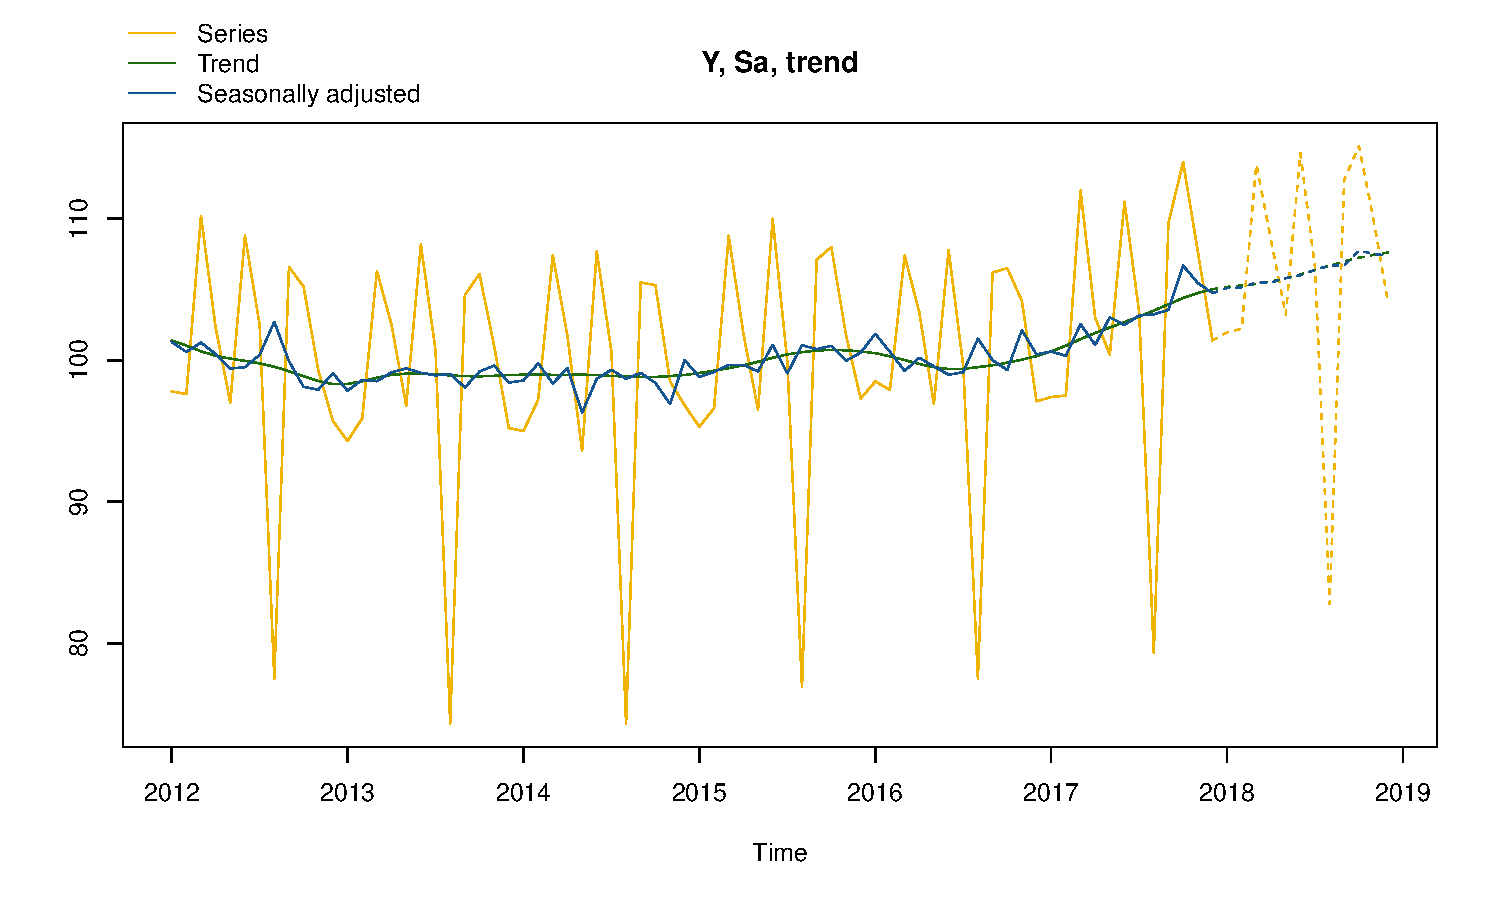
\includegraphics{img/markdown-unnamed-chunk-16-1.pdf}

\end{frame}

\begin{frame}[fragile]{CVS-CJO : exemples (8/8)}
\protect\hypertarget{cvs-cjo-exemples-88}{}

\footnotesize

\begin{Shaded}
\begin{Highlighting}[]
\NormalTok{x13_mod}\OperatorTok{$}\NormalTok{diagnostics}
\end{Highlighting}
\end{Shaded}

\begin{verbatim}
##  Relative contribution of the components to the stationary
##  portion of the variance in the original series,
##  after the removal of the long term trend 
##  Trend computed by Hodrick-Prescott filter (cycle length = 8.0 years)
##            Component
##  Cycle         1.557
##  Seasonal     39.219
##  Irregular     0.362
##  TD & Hol.     0.018
##  Others       61.971
##  Total       103.128
## 
##  Combined test in the entire series 
##  Non parametric tests for stable seasonality
##                                                           P.value
##    Kruskall-Wallis test                                      0.000
##    Test for the presence of seasonality assuming stability   0.000
##    Evolutive seasonality test                                0.032
##  
##  Identifiable seasonality present
## 
##  Residual seasonality tests 
##                                       P.value
##  qs test on sa                          1.000
##  qs test on i                           1.000
##  f-test on sa (seasonal dummies)        0.997
##  f-test on i (seasonal dummies)         0.965
##  Residual seasonality (entire series)   0.993
##  Residual seasonality (last 3 years)    0.922
##  f-test on sa (td)                      0.001
##  f-test on i (td)                       0.006
\end{verbatim}

\end{frame}

\hypertarget{manipuler-des-workspaces}{%
\subsection{Manipuler des workspaces}\label{manipuler-des-workspaces}}

\begin{frame}[fragile]{Exporter un workspace}
\protect\hypertarget{exporter-un-workspace}{}

\footnotesize

\begin{Shaded}
\begin{Highlighting}[]
\NormalTok{wk <-}\StringTok{ }\KeywordTok{new_workspace}\NormalTok{()}
\KeywordTok{new_multiprocessing}\NormalTok{(wk, }\DataTypeTok{name =} \StringTok{"MP-1"}\NormalTok{)}
\KeywordTok{add_sa_item}\NormalTok{(wk, }\DataTypeTok{multiprocessing =} \StringTok{"MP-1"}\NormalTok{,}
            \DataTypeTok{sa_obj =}\NormalTok{ x13_mod, }\DataTypeTok{name =}  \StringTok{"SA with X13 model 1 "}\NormalTok{)}
\KeywordTok{add_sa_item}\NormalTok{(wk, }\DataTypeTok{multiprocessing =}  \StringTok{"MP-1"}\NormalTok{,}
            \DataTypeTok{sa_obj =}\NormalTok{ ts_mod, }\DataTypeTok{name =} \StringTok{"SA with TramoSeats model 1"}\NormalTok{)}
\KeywordTok{save_workspace}\NormalTok{(wk, }\StringTok{"workspace.xml"}\NormalTok{)}
\end{Highlighting}
\end{Shaded}

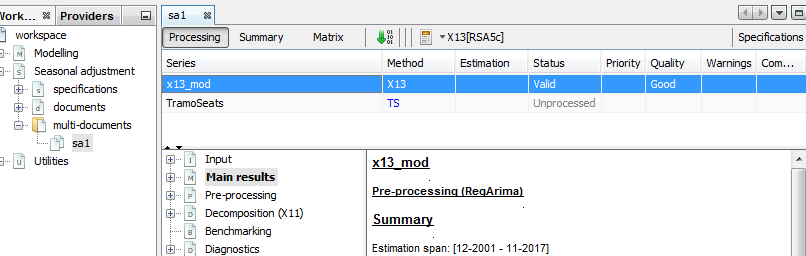
\includegraphics{img/workspace.png}

\end{frame}

\begin{frame}[fragile]{Importer un workspace (1/3)}
\protect\hypertarget{importer-un-workspace-13}{}

\footnotesize

\begin{Shaded}
\begin{Highlighting}[]
\NormalTok{wk <-}\StringTok{ }\KeywordTok{load_workspace}\NormalTok{(}\StringTok{"workspace.xml"}\NormalTok{)}
\KeywordTok{get_ts}\NormalTok{(wk)}
\end{Highlighting}
\end{Shaded}

\begin{verbatim}
## $`MP-1`
## $`MP-1`$`SA with X13 model 1 `
##        Jan   Feb   Mar   Apr   May   Jun   Jul   Aug   Sep   Oct   Nov
## 1990  90.5  92.6 101.9  95.2  92.1 103.3  91.8  65.5  99.0 102.8  94.3
## 1991  90.9  89.6  99.9  93.3  88.3 103.0  89.7  65.1  98.2 100.8  95.8
## 1992  89.4  89.0  99.5  93.0  89.1 101.3  89.4  64.1  94.9  98.6  92.2
## 1993  85.3  84.3  93.2  87.8  83.5  95.4  86.2  60.1  92.1  95.8  88.1
## 1994  84.9  84.0  94.1  90.1  86.8 100.4  90.8  64.5  96.8 101.0  96.6
## 1995  90.4  90.5 100.4  94.5  89.7 103.7  93.8  65.5  99.7 101.8  94.6
## 1996  90.3  88.8 100.7  93.8  91.2 104.4  92.3  67.2 100.2 102.3  96.9
## 1997  90.5  91.6 104.0  99.7  93.9 108.8  98.2  73.4 105.8 111.8 102.4
## 1998  99.2  99.0 109.4 103.0 100.7 114.8 104.9  73.3 109.6 112.7 105.9
## 1999 100.5  98.6 111.8 104.3 101.3 117.4 106.6  74.9 113.4 118.2 110.9
## 2000 104.8 104.9 118.9 110.2 108.0 122.5 111.8  80.5 117.5 121.7 114.3
## 2001 108.8 109.2 123.7 111.8 108.4 124.7 111.1  84.2 117.8 121.0 111.6
## 2002 106.6 107.0 121.4 112.8 106.4 122.2 109.7  82.3 117.1 118.7 113.0
## 2003 105.4 105.7 120.1 111.1 102.8 118.3 108.8  78.7 115.9 119.9 110.8
## 2004 105.8 107.0 120.0 112.1 105.8 123.6 112.0  78.4 120.0 122.0 112.0
## 2005 109.1 106.7 117.9 113.5 106.8 122.3 110.3  80.0 121.4 118.4 115.2
## 2006 107.3 106.3 121.9 112.5 110.8 126.7 112.5  82.5 122.2 121.9 113.7
## 2007 109.5 110.0 123.8 114.2 112.6 127.0 115.2  85.7 121.2 124.7 115.2
## 2008 111.4 112.2 123.0 116.8 108.4 122.1 112.6  81.9 117.3 116.3 102.4
## 2009  91.7  90.4 100.1  93.2  91.4 105.5  96.8  71.6 104.5 104.8  99.3
## 2010  93.7  93.5 106.8  99.9  96.9 108.9 101.7  73.2 107.2 108.2 102.5
## 2011 100.4 102.0 112.0 103.7 102.9 111.3 105.0  76.6 108.4 109.7 106.0
## 2012  97.8  97.6 110.2 102.3  97.0 108.8 102.5  77.5 106.6 105.2  99.3
## 2013  94.3  95.9 106.3 102.5  96.8 108.2 100.7  74.3 104.6 106.1 101.0
## 2014  95.0  97.2 107.4 101.7  93.6 107.7 100.6  74.3 105.5 105.3  98.5
## 2015  95.3  96.6 108.8 101.9  96.5 110.0  99.9  76.9 107.1 108.0 101.8
## 2016  98.5  97.9 107.4 103.4  96.9 107.8  99.6  77.5 106.2 106.5 104.2
## 2017  97.4  97.5 112.0 103.0 100.4 111.2 103.4  79.3 109.7 114.0 107.7
##        Dec
## 1990  93.1
## 1991  93.2
## 1992  90.5
## 1993  88.3
## 1994  96.3
## 1995  98.1
## 1996  97.2
## 1997 105.4
## 1998 105.1
## 1999 109.8
## 2000 115.5
## 2001 109.2
## 2002 106.4
## 2003 107.9
## 2004 108.4
## 2005 109.8
## 2006 111.7
## 2007 111.0
## 2008  97.8
## 2009  92.9
## 2010  97.9
## 2011  98.4
## 2012  95.7
## 2013  95.2
## 2014  96.8
## 2015  97.3
## 2016  97.1
## 2017 101.4
## 
## $`MP-1`$`SA with TramoSeats model 1`
##        Jan   Feb   Mar   Apr   May   Jun   Jul   Aug   Sep   Oct   Nov
## 1990  90.5  92.6 101.9  95.2  92.1 103.3  91.8  65.5  99.0 102.8  94.3
## 1991  90.9  89.6  99.9  93.3  88.3 103.0  89.7  65.1  98.2 100.8  95.8
## 1992  89.4  89.0  99.5  93.0  89.1 101.3  89.4  64.1  94.9  98.6  92.2
## 1993  85.3  84.3  93.2  87.8  83.5  95.4  86.2  60.1  92.1  95.8  88.1
## 1994  84.9  84.0  94.1  90.1  86.8 100.4  90.8  64.5  96.8 101.0  96.6
## 1995  90.4  90.5 100.4  94.5  89.7 103.7  93.8  65.5  99.7 101.8  94.6
## 1996  90.3  88.8 100.7  93.8  91.2 104.4  92.3  67.2 100.2 102.3  96.9
## 1997  90.5  91.6 104.0  99.7  93.9 108.8  98.2  73.4 105.8 111.8 102.4
## 1998  99.2  99.0 109.4 103.0 100.7 114.8 104.9  73.3 109.6 112.7 105.9
## 1999 100.5  98.6 111.8 104.3 101.3 117.4 106.6  74.9 113.4 118.2 110.9
## 2000 104.8 104.9 118.9 110.2 108.0 122.5 111.8  80.5 117.5 121.7 114.3
## 2001 108.8 109.2 123.7 111.8 108.4 124.7 111.1  84.2 117.8 121.0 111.6
## 2002 106.6 107.0 121.4 112.8 106.4 122.2 109.7  82.3 117.1 118.7 113.0
## 2003 105.4 105.7 120.1 111.1 102.8 118.3 108.8  78.7 115.9 119.9 110.8
## 2004 105.8 107.0 120.0 112.1 105.8 123.6 112.0  78.4 120.0 122.0 112.0
## 2005 109.1 106.7 117.9 113.5 106.8 122.3 110.3  80.0 121.4 118.4 115.2
## 2006 107.3 106.3 121.9 112.5 110.8 126.7 112.5  82.5 122.2 121.9 113.7
## 2007 109.5 110.0 123.8 114.2 112.6 127.0 115.2  85.7 121.2 124.7 115.2
## 2008 111.4 112.2 123.0 116.8 108.4 122.1 112.6  81.9 117.3 116.3 102.4
## 2009  91.7  90.4 100.1  93.2  91.4 105.5  96.8  71.6 104.5 104.8  99.3
## 2010  93.7  93.5 106.8  99.9  96.9 108.9 101.7  73.2 107.2 108.2 102.5
## 2011 100.4 102.0 112.0 103.7 102.9 111.3 105.0  76.6 108.4 109.7 106.0
## 2012  97.8  97.6 110.2 102.3  97.0 108.8 102.5  77.5 106.6 105.2  99.3
## 2013  94.3  95.9 106.3 102.5  96.8 108.2 100.7  74.3 104.6 106.1 101.0
## 2014  95.0  97.2 107.4 101.7  93.6 107.7 100.6  74.3 105.5 105.3  98.5
## 2015  95.3  96.6 108.8 101.9  96.5 110.0  99.9  76.9 107.1 108.0 101.8
## 2016  98.5  97.9 107.4 103.4  96.9 107.8  99.6  77.5 106.2 106.5 104.2
## 2017  97.4  97.5 112.0 103.0 100.4 111.2 103.4  79.3 109.7 114.0 107.7
##        Dec
## 1990  93.1
## 1991  93.2
## 1992  90.5
## 1993  88.3
## 1994  96.3
## 1995  98.1
## 1996  97.2
## 1997 105.4
## 1998 105.1
## 1999 109.8
## 2000 115.5
## 2001 109.2
## 2002 106.4
## 2003 107.9
## 2004 108.4
## 2005 109.8
## 2006 111.7
## 2007 111.0
## 2008  97.8
## 2009  92.9
## 2010  97.9
## 2011  98.4
## 2012  95.7
## 2013  95.2
## 2014  96.8
## 2015  97.3
## 2016  97.1
## 2017 101.4
\end{verbatim}

\end{frame}

\begin{frame}{Importer un workspace (2/3)}
\protect\hypertarget{importer-un-workspace-23}{}

\animategraphics[loop, autoplay, width=\linewidth]{2.5}{img/gif/import_model/}{1}{114}

\end{frame}

\begin{frame}[fragile]{Importer un workspace (3/3)}
\protect\hypertarget{importer-un-workspace-33}{}

\footnotesize

\begin{Shaded}
\begin{Highlighting}[]
\KeywordTok{compute}\NormalTok{(wk) }\CommentTok{# Important to get the Sa model}
\NormalTok{models <-}\StringTok{ }\KeywordTok{get_model}\NormalTok{(wk) }\CommentTok{# A progress bar is printed by default}
\end{Highlighting}
\end{Shaded}

\begin{verbatim}
## Multiprocessing 1 on 1:
## 
  |                                                                       
  |                                                                 |   0%
  |                                                                       
  |================================                                 |  50%
  |                                                                       
  |=================================================================| 100%
\end{verbatim}

\begin{Shaded}
\begin{Highlighting}[]
\CommentTok{# To extract only one model}
\NormalTok{mp <-}\StringTok{ }\KeywordTok{get_object}\NormalTok{(wk, }\DecValTok{1}\NormalTok{)}
\KeywordTok{count}\NormalTok{(mp)}
\end{Highlighting}
\end{Shaded}

\begin{verbatim}
## [1] 2
\end{verbatim}

\begin{Shaded}
\begin{Highlighting}[]
\NormalTok{sa2 <-}\StringTok{ }\KeywordTok{get_object}\NormalTok{(mp,}\DecValTok{2}\NormalTok{)}
\KeywordTok{get_name}\NormalTok{(sa2)}
\end{Highlighting}
\end{Shaded}

\begin{verbatim}
## [1] "SA with TramoSeats model 1"
\end{verbatim}

\begin{Shaded}
\begin{Highlighting}[]
\NormalTok{mod <-}\StringTok{ }\KeywordTok{get_model}\NormalTok{(wk, sa2)}
\end{Highlighting}
\end{Shaded}

\begin{verbatim}
## Multiprocessing 1 on 1:
## 
  |                                                                       
  |                                                                 |   0%
  |                                                                       
  |================================                                 |  50%
  |                                                                       
  |=================================================================| 100%
\end{verbatim}

\end{frame}

\hypertarget{comment-installer-le-package}{%
\subsection{Comment installer le package
?}\label{comment-installer-le-package}}

\begin{frame}[fragile]{Comment installer le package ?}
\protect\hypertarget{comment-installer-le-package-1}{}

Package disponible sur \large\faGithub\normalsize:
\url{https://github.com/jdemetra/rjdemetra}

Il a sa propre page web : \url{https://jdemetra.github.io/rjdemetra/}

Peut être installé depuis le CRAN:

\begin{Shaded}
\begin{Highlighting}[]
\KeywordTok{install.packages}\NormalTok{(}\StringTok{"RJDemetra"}\NormalTok{)}
\end{Highlighting}
\end{Shaded}

Ou depuis github (version de développement):

\begin{Shaded}
\begin{Highlighting}[]
\NormalTok{devtools}\OperatorTok{::}\KeywordTok{install_github}\NormalTok{(}\StringTok{"jdemetra/rjdemetra"}\NormalTok{)}
\end{Highlighting}
\end{Shaded}

\bcinfo Il faut Java8 : à l'Insee, il faut utiliser une version portable
de Java et configurer le \texttt{JAVA\_HOME}. Sous AUS :

\begin{Shaded}
\begin{Highlighting}[]
\KeywordTok{Sys.setenv}\NormalTok{(}\DataTypeTok{JAVA_HOME=}\StringTok{'Y:\textbackslash{}Logiciels\textbackslash{}J8Px64\textbackslash{}Java64'}\NormalTok{)}
\end{Highlighting}
\end{Shaded}

\end{frame}

\hypertarget{developpements-futurs}{%
\subsection{Développements futurs}\label{developpements-futurs}}

\begin{frame}{What's next? \bcpanchant (1/2)}
\protect\hypertarget{whats-next-12}{}

Documentation:

\begin{itemize}
\item
  Vignette/article pour Journal of Statistical Software
\item
  Guide pour installer le package avec une version portable de Java
\item
  Cheat sheet
\end{itemize}

\end{frame}

\begin{frame}[fragile]{What's next? \bcpanchant (2/2)}
\protect\hypertarget{whats-next-22}{}

Package:

\begin{itemize}
\item
  Récupérer uniquement l'objet Java Java de la CVS-CJO (pour réduire le
  temps de calcul/personnaliser l'output) \(\rightarrow\) dans la
  version GitHub : \texttt{jx13}, \texttt{jregarima}\ldots{}
\item
  Possibilité d'utiliser des régresseurs de calendrier personnalisés
  user-defined calendar regressors \(\rightarrow\) dans la version
  GitHub
\item
  Possibilité de ``rafraîchir'' le modèle (JD+ 3.0.0)
\end{itemize}

\end{frame}

\begin{frame}{Performance}
\protect\hypertarget{performance}{}

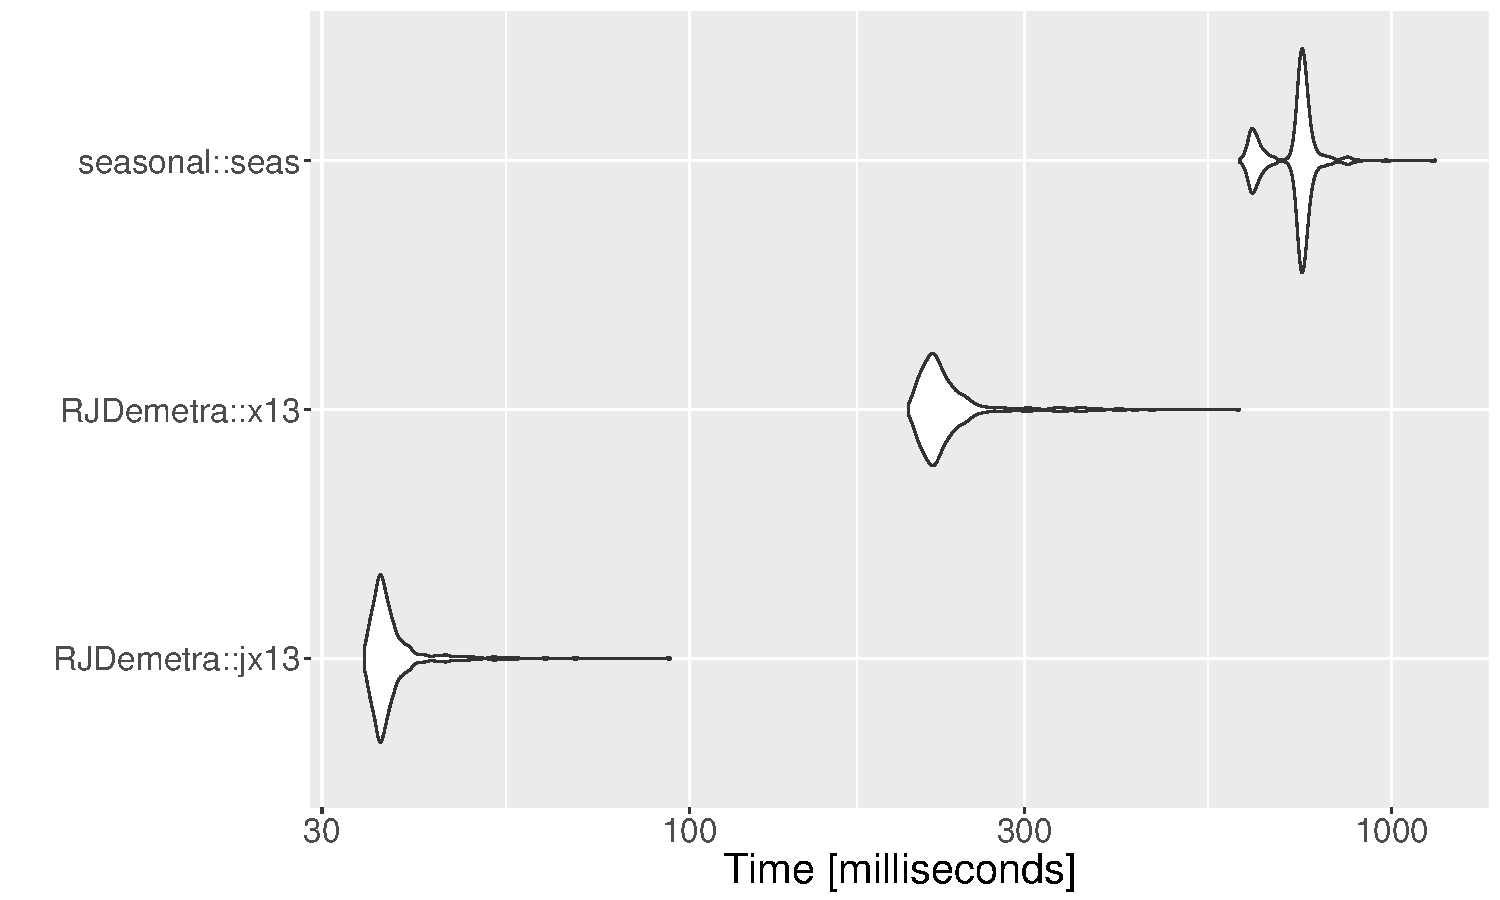
\includegraphics{img/markdown-unnamed-chunk-24-1.pdf}

\end{frame}

\hypertarget{utilisation-de-rjdemetra-pour-ameliorer-la-production}{%
\section{Utilisation de RJDemetra pour améliorer la
production}\label{utilisation-de-rjdemetra-pour-ameliorer-la-production}}

\hypertarget{autour-de-rjdemetra}{%
\subsection{Autour de RJDemetra}\label{autour-de-rjdemetra}}

\begin{frame}{Exemples d'utilisation de RJDemetra}
\protect\hypertarget{exemples-dutilisation-de-rjdemetra}{}

\begin{itemize}
\tightlist
\item
  rjdqa (expérimental, sans documentation) : package pour aider à
  évaluer la qualité de la désaisonnalisation (tableau de bord et bilan
  qualité)
\end{itemize}

\faGithub{} \url{https://github.com/AQLT/rjdqa}

\begin{itemize}
\tightlist
\item
  persephone (expérimental) : faciliter la production de séries CVS-CJO
  au sein de l'institut (graphiques interactifs, tableaux de
  bord\ldots{})
\end{itemize}

\faGithub{} \url{https://github.com/statistikat/persephone}

\begin{itemize}
\tightlist
\item
  ggdemetra (très expérimental) : intégrer la désaisonnalisation à
  ggplot2
\end{itemize}

\faGithub{} \url{https://github.com/AQLT/ggdemetra}

\begin{itemize}
\item
  Sujets non explorés : comparaison approches directes et indirectes,
  analyse des révisions, etc.
\item
  Réalisations d'études : Ladiray D., Quartier-la-Tente A., ``Du bon
  usage des modèles Reg-ARIMA en désaisonnalisation'', JMS 2018
\end{itemize}

\end{frame}

\begin{frame}[fragile]{rjdqa}
\protect\hypertarget{rjdqa}{}

\footnotesize

\begin{Shaded}
\begin{Highlighting}[]
\KeywordTok{plot}\NormalTok{(rjdqa}\OperatorTok{::}\KeywordTok{sa_dashboard}\NormalTok{(x13_mod))}
\end{Highlighting}
\end{Shaded}

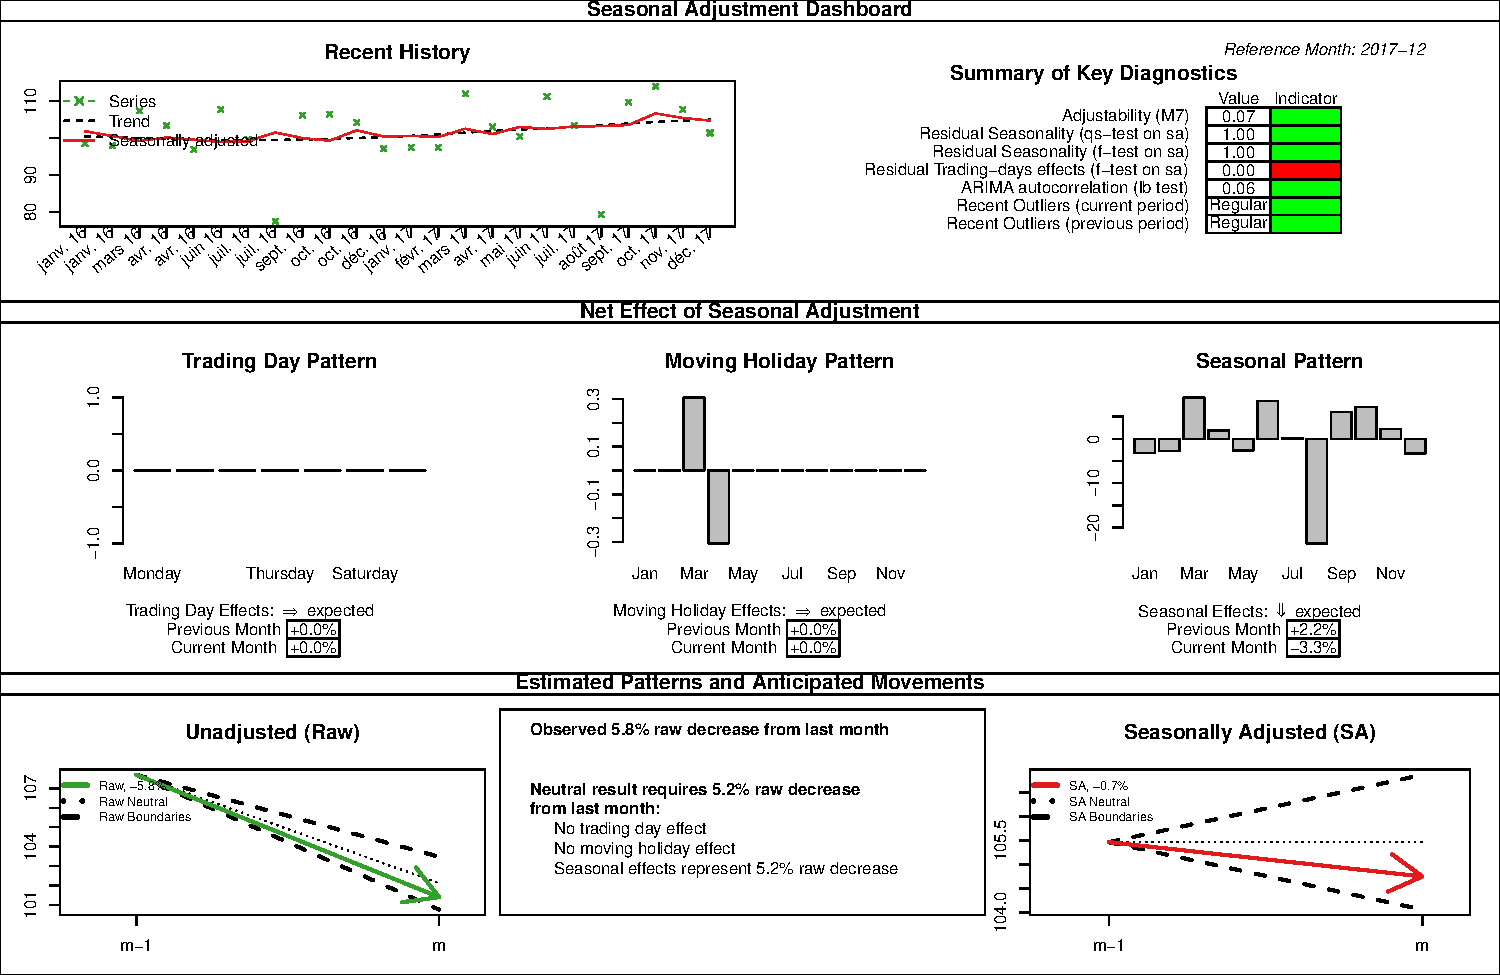
\includegraphics{img/markdown-unnamed-chunk-25-1.pdf}

\end{frame}

\begin{frame}{persephone}
\protect\hypertarget{persephone}{}

\animategraphics[loop, autoplay, width=0.9\linewidth]{3}{img/gif/persephone/}{1}{167}

\end{frame}

\begin{frame}[fragile]{ggdemetra : extension de ggplot2}
\protect\hypertarget{ggdemetra-extension-de-ggplot2}{}

Exemple de création de fonction \texttt{stat\_} pour \texttt{ggplot2} et
effectuer de la désaisonnalisation ``on the fly''

\url{https://ggplot2.tidyverse.org/articles/extending-ggplot2.html}

\footnotesize

\begin{Shaded}
\begin{Highlighting}[]
\KeywordTok{library}\NormalTok{(ggplot2)}
\KeywordTok{library}\NormalTok{(ggdemetra)}
\CommentTok{# IPI France}
\NormalTok{myseries_data <-}\StringTok{ }\KeywordTok{data.frame}\NormalTok{(}\DataTypeTok{x =} \KeywordTok{as.numeric}\NormalTok{(}\KeywordTok{time}\NormalTok{(ipi_c_eu)),}
                            \DataTypeTok{y =} \KeywordTok{as.numeric}\NormalTok{(ipi_c_eu[, }\StringTok{"FR"}\NormalTok{]))}

\CommentTok{# IPI France et Italie}
\NormalTok{myseries_data2 <-}\StringTok{ }\KeywordTok{rbind}\NormalTok{(}\KeywordTok{data.frame}\NormalTok{(}\DataTypeTok{x =} \KeywordTok{as.numeric}\NormalTok{(}\KeywordTok{time}\NormalTok{(ipi_c_eu)),}
                                   \DataTypeTok{y =} \KeywordTok{as.numeric}\NormalTok{(ipi_c_eu[, }\StringTok{"FR"}\NormalTok{]),}
                                   \DataTypeTok{pays =} \StringTok{"FR"}\NormalTok{, }\DataTypeTok{stringsAsFactors =} \OtherTok{FALSE}\NormalTok{),}
                        \KeywordTok{data.frame}\NormalTok{(}\DataTypeTok{x =} \KeywordTok{as.numeric}\NormalTok{(}\KeywordTok{time}\NormalTok{(ipi_c_eu)),}
                                   \DataTypeTok{y =} \KeywordTok{as.numeric}\NormalTok{(ipi_c_eu[, }\StringTok{"IT"}\NormalTok{]),}
                                   \DataTypeTok{pays =} \StringTok{"IT"}\NormalTok{, }\DataTypeTok{stringsAsFactors =} \OtherTok{FALSE}\NormalTok{))}
\NormalTok{p1 <-}\StringTok{ }\KeywordTok{ggplot}\NormalTok{(myseries_data, }\KeywordTok{aes}\NormalTok{(x, y)) }\OperatorTok{+}\StringTok{ }
\StringTok{  }\KeywordTok{geom_line}\NormalTok{()}
\end{Highlighting}
\end{Shaded}

\end{frame}

\begin{frame}[fragile]{ggdemetra : extension de ggplot2}
\protect\hypertarget{ggdemetra-extension-de-ggplot2-1}{}

\begin{Shaded}
\begin{Highlighting}[]
\NormalTok{p1}
\end{Highlighting}
\end{Shaded}

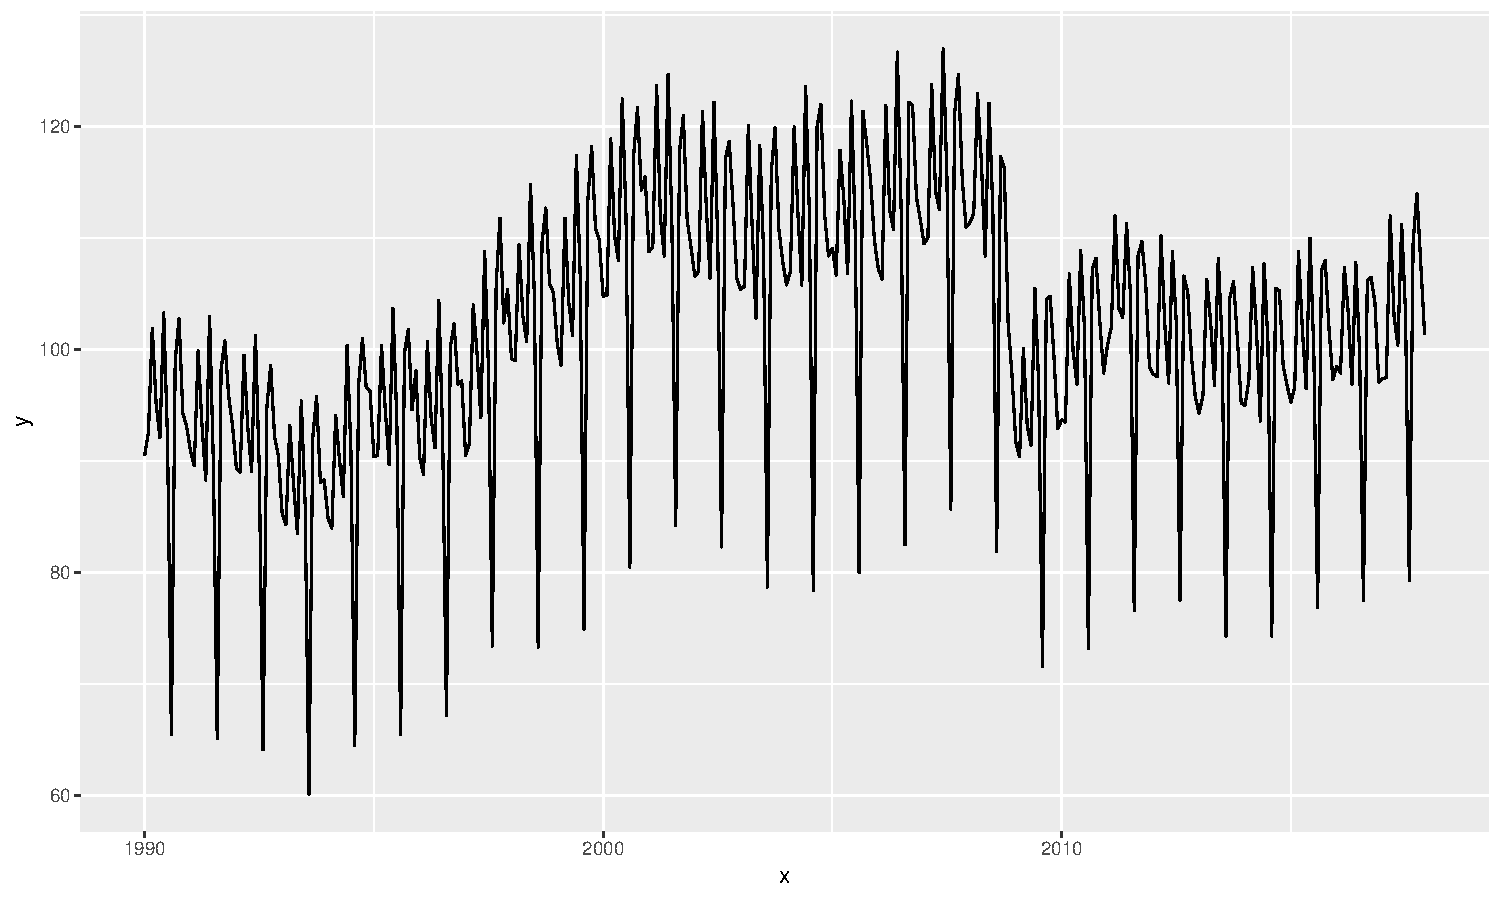
\includegraphics{img/markdown-unnamed-chunk-27-1.pdf}

\end{frame}

\begin{frame}[fragile]{ggdemetra : extension de ggplot2}
\protect\hypertarget{ggdemetra-extension-de-ggplot2-2}{}

Pour rajouter la série désaisonnalisée et la tendance :

\begin{Shaded}
\begin{Highlighting}[]
\NormalTok{p2 <-}\StringTok{ }\KeywordTok{ggplot}\NormalTok{(myseries_data, }\KeywordTok{aes}\NormalTok{(x, y)) }\OperatorTok{+}\StringTok{ }
\StringTok{  }\KeywordTok{geom_line}\NormalTok{() }\OperatorTok{+}\StringTok{ }
\StringTok{  }\KeywordTok{stat_sa}\NormalTok{(}\DataTypeTok{colour =} \StringTok{"red"}\NormalTok{, }\DataTypeTok{component =} \StringTok{"sa"}\NormalTok{,}
          \DataTypeTok{spec =} \StringTok{"RSA3"}\NormalTok{) }\OperatorTok{+}
\StringTok{  }\KeywordTok{stat_sa}\NormalTok{(}\DataTypeTok{colour =} \StringTok{"green"}\NormalTok{, }\DataTypeTok{component =} \StringTok{"t"}\NormalTok{,}
          \DataTypeTok{spec =} \StringTok{"RSA3"}\NormalTok{)}
\end{Highlighting}
\end{Shaded}

Pour faire la désaisonnalisation sur plusieurs séries :

\begin{Shaded}
\begin{Highlighting}[]
\NormalTok{p3 <-}\StringTok{ }\KeywordTok{ggplot}\NormalTok{(myseries_data2,}
             \KeywordTok{aes}\NormalTok{(x, y, }\DataTypeTok{colour =}\NormalTok{ pays, }\DataTypeTok{group =}\NormalTok{ pays)) }\OperatorTok{+}\StringTok{ }
\StringTok{  }\KeywordTok{geom_line}\NormalTok{() }\OperatorTok{+}\StringTok{ }
\StringTok{  }\KeywordTok{stat_sa}\NormalTok{(}\DataTypeTok{colour =} \StringTok{"black"}\NormalTok{, }\DataTypeTok{component =} \StringTok{"sa"}\NormalTok{,}
          \DataTypeTok{spec =} \StringTok{"RSA0"}\NormalTok{)}
\end{Highlighting}
\end{Shaded}

\end{frame}

\begin{frame}[fragile]{ggdemetra : extension de ggplot2}
\protect\hypertarget{ggdemetra-extension-de-ggplot2-3}{}

\begin{Shaded}
\begin{Highlighting}[]
\NormalTok{p2}
\end{Highlighting}
\end{Shaded}

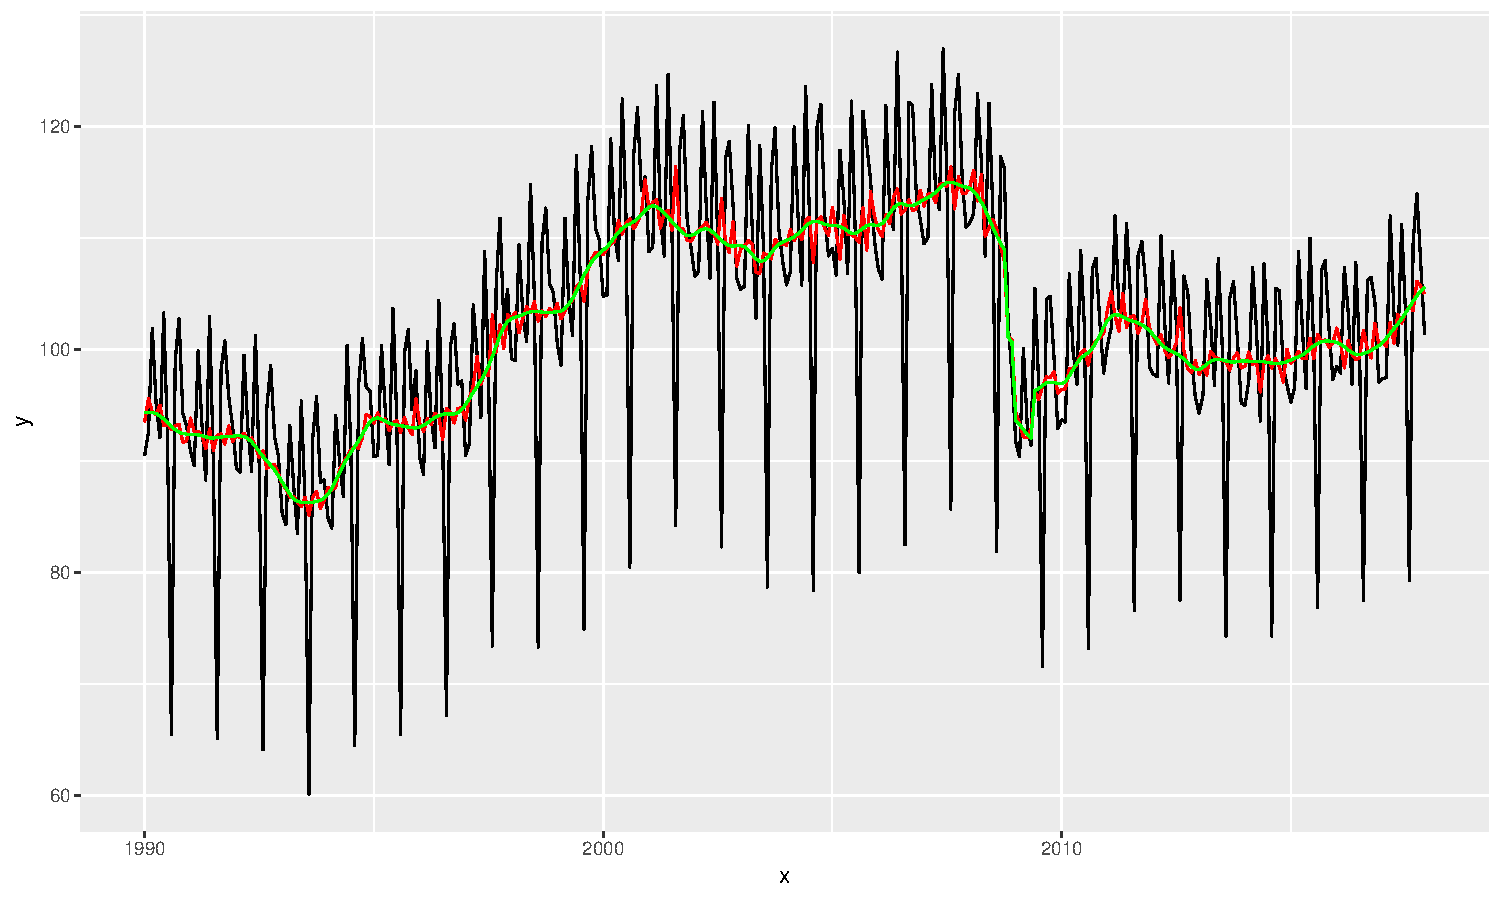
\includegraphics{img/markdown-unnamed-chunk-30-1.pdf}

\end{frame}

\begin{frame}[fragile]{ggdemetra : extension de ggplot2}
\protect\hypertarget{ggdemetra-extension-de-ggplot2-4}{}

\begin{Shaded}
\begin{Highlighting}[]
\NormalTok{p3}
\end{Highlighting}
\end{Shaded}

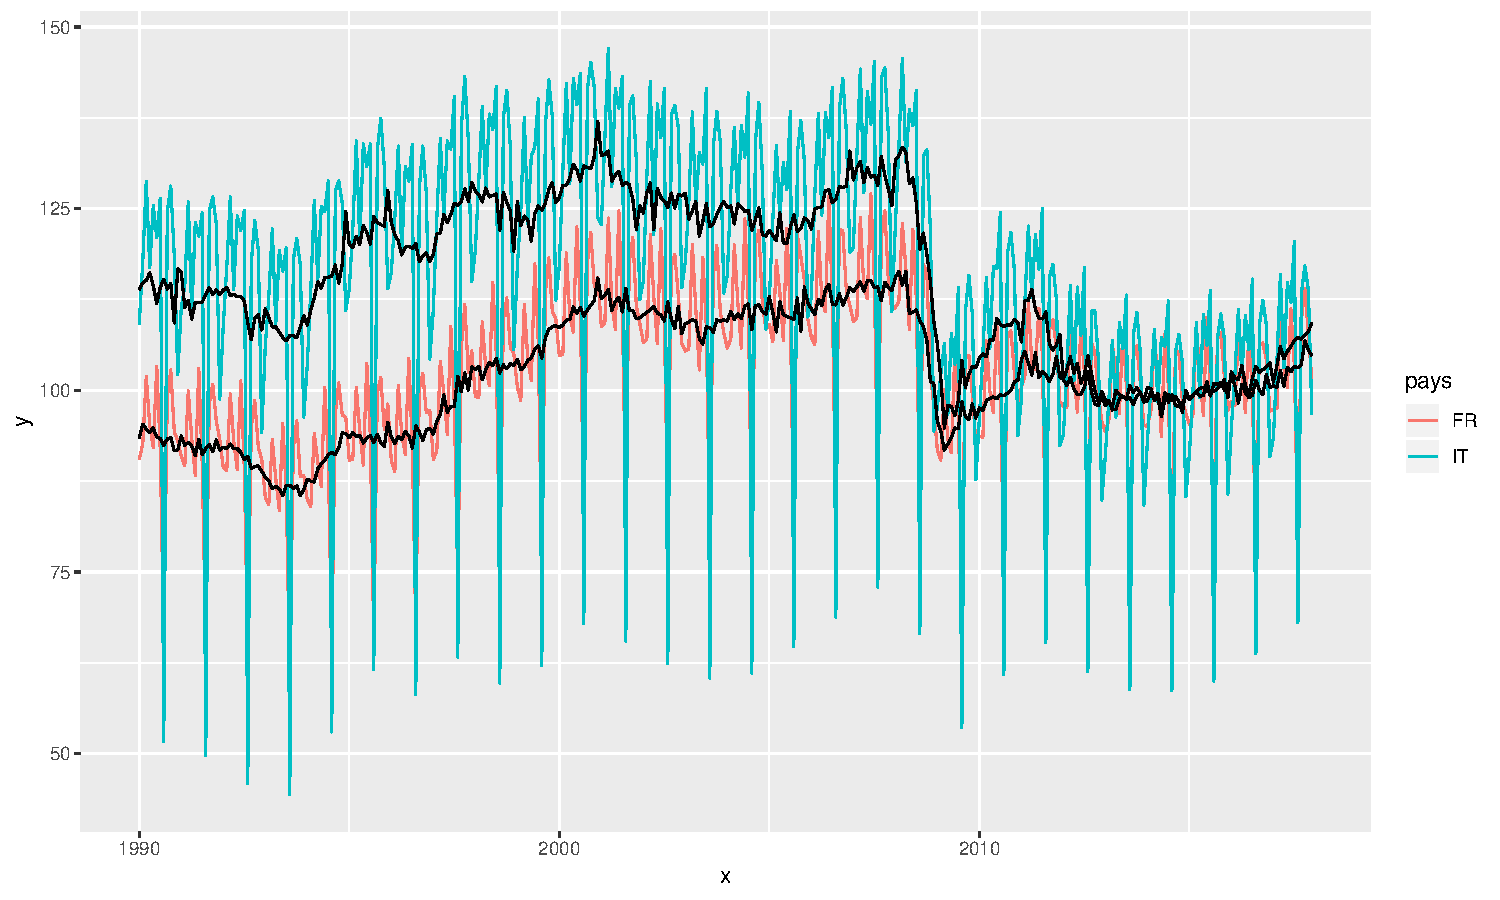
\includegraphics{img/markdown-unnamed-chunk-31-1.pdf}

\end{frame}

\begin{frame}[fragile]{ggdemetra : extension de ggplot2}
\protect\hypertarget{ggdemetra-extension-de-ggplot2-5}{}

\footnotesize

\begin{Shaded}
\begin{Highlighting}[]
\NormalTok{p2 }\OperatorTok{+}\StringTok{ }\KeywordTok{stat_outliers}\NormalTok{(}\DataTypeTok{color =} \StringTok{"red"}\NormalTok{, }\DataTypeTok{vjust =} \DecValTok{4}\NormalTok{, }\DataTypeTok{ylim =} \KeywordTok{c}\NormalTok{(}\OtherTok{NA}\NormalTok{, }\DecValTok{80}\NormalTok{), }\DataTypeTok{force =} \DecValTok{10}\NormalTok{,}
                   \DataTypeTok{arrow =} \KeywordTok{arrow}\NormalTok{(}\DataTypeTok{length =} \KeywordTok{unit}\NormalTok{(}\FloatTok{0.03}\NormalTok{, }\StringTok{"npc"}\NormalTok{),}
                                 \DataTypeTok{type =} \StringTok{"closed"}\NormalTok{, }\DataTypeTok{ends =} \StringTok{"last"}\NormalTok{))   }\OperatorTok{+}
\StringTok{  }\KeywordTok{geom_label_arima}\NormalTok{(}\DataTypeTok{x =} \OperatorTok{-}\StringTok{ }\OtherTok{Inf}\NormalTok{, }\DataTypeTok{y =} \OperatorTok{-}\OtherTok{Inf}\NormalTok{, }\DataTypeTok{vjust =} \DecValTok{-1}\NormalTok{, }\DataTypeTok{hjust =} \FloatTok{-0.1}\NormalTok{)}
\end{Highlighting}
\end{Shaded}

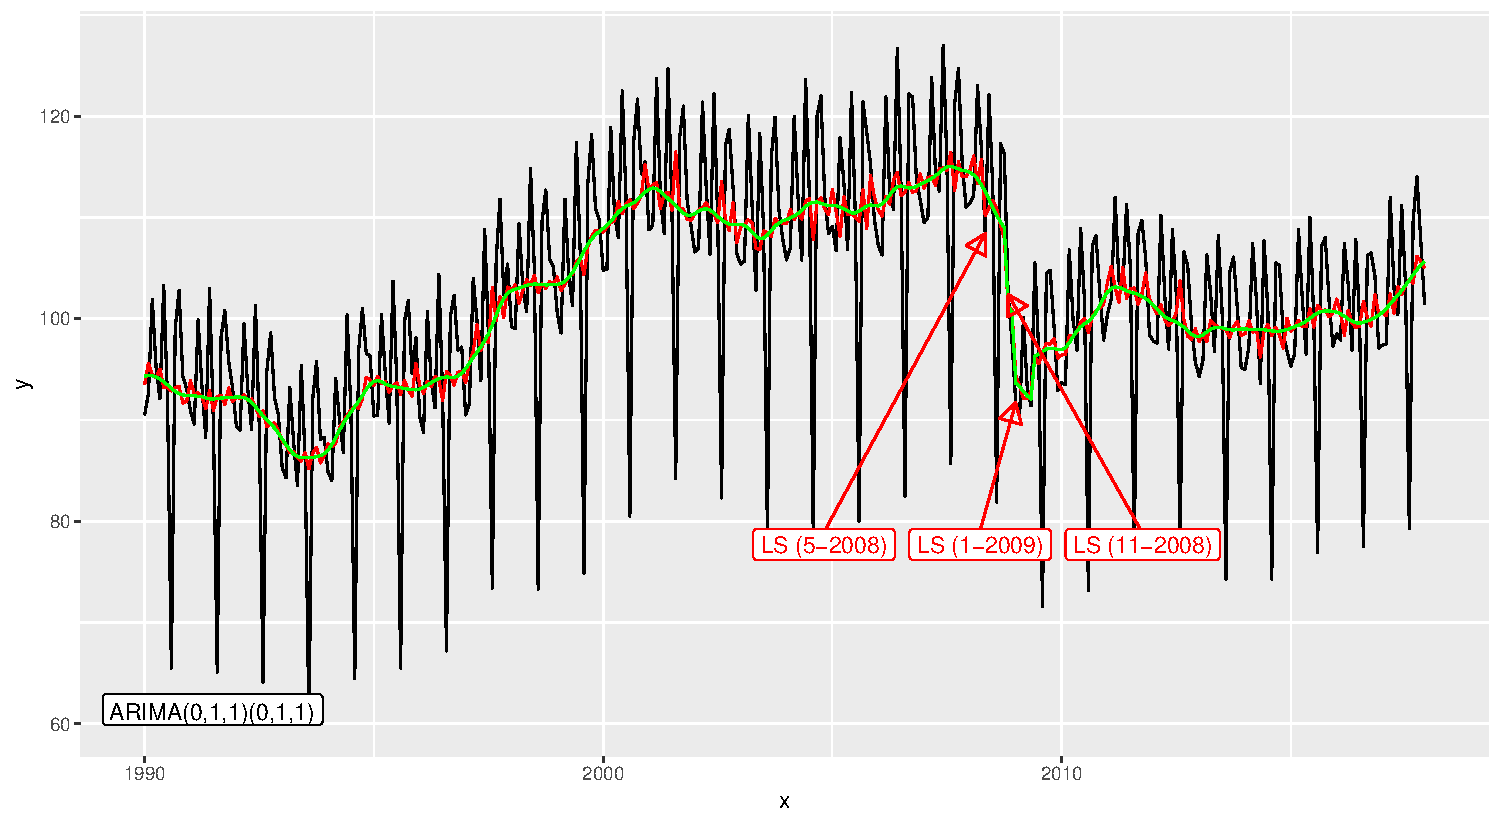
\includegraphics{img/markdown-unnamed-chunk-32-1.pdf}

\end{frame}

\begin{frame}[fragile]{ggdemetra : extension de ggplot2}
\protect\hypertarget{ggdemetra-extension-de-ggplot2-6}{}

Deux fonctions à écrire : \texttt{stat\_sa} et \texttt{StatSa}

\footnotesize

\begin{Shaded}
\begin{Highlighting}[]
\NormalTok{stat_sa <-}\StringTok{ }\ControlFlowTok{function}\NormalTok{(}\DataTypeTok{mapping =} \OtherTok{NULL}\NormalTok{, }\DataTypeTok{data =} \OtherTok{NULL}\NormalTok{, }\DataTypeTok{geom =} \StringTok{"line"}\NormalTok{,}
                    \DataTypeTok{position =} \StringTok{"identity"}\NormalTok{, }\DataTypeTok{show.legend =} \OtherTok{NA}\NormalTok{, }
                    \DataTypeTok{inherit.aes =} \OtherTok{TRUE}\NormalTok{,}
                    \DataTypeTok{method =} \KeywordTok{c}\NormalTok{(}\StringTok{"x13"}\NormalTok{,}\StringTok{"tramoseats"}\NormalTok{),}
                    \DataTypeTok{frequency =} \DecValTok{12}\NormalTok{, }\DataTypeTok{spec =} \OtherTok{NULL}
                    \DataTypeTok{component =} \StringTok{"sa"}\NormalTok{,}
\NormalTok{                    ...) \{}
\NormalTok{    ggplot2}\OperatorTok{::}\KeywordTok{layer}\NormalTok{(}
        \DataTypeTok{stat =}\NormalTok{ StatSa, }\DataTypeTok{data =}\NormalTok{ data, }\DataTypeTok{mapping =}\NormalTok{ mapping, }\DataTypeTok{geom =}\NormalTok{ geom, }
        \DataTypeTok{position =}\NormalTok{ position, }\DataTypeTok{show.legend =}\NormalTok{ show.legend,}
        \DataTypeTok{inherit.aes =}\NormalTok{ inherit.aes,}
        \DataTypeTok{params =} \KeywordTok{list}\NormalTok{(}\DataTypeTok{method =}\NormalTok{ method, }\DataTypeTok{frequency =}\NormalTok{ frequency,}
                      \DataTypeTok{component =}\NormalTok{ component,}
                      \DataTypeTok{spec =}\NormalTok{ spec, ...)}
\NormalTok{    )}
\NormalTok{\}}
\end{Highlighting}
\end{Shaded}

\end{frame}

\begin{frame}[fragile]{ggdemetra : extension de ggplot2}
\protect\hypertarget{ggdemetra-extension-de-ggplot2-7}{}

\footnotesize

\begin{Shaded}
\begin{Highlighting}[]
\NormalTok{StatSa <-}\StringTok{ }\KeywordTok{ggproto}\NormalTok{(}\StringTok{"StatSa"}\NormalTok{, Stat, }\DataTypeTok{required_aes =} \KeywordTok{c}\NormalTok{(}\StringTok{"x"}\NormalTok{, }\StringTok{"y"}\NormalTok{),}
                  \DataTypeTok{compute_group =} \ControlFlowTok{function}\NormalTok{(data, scales,}
                                           \DataTypeTok{method =} \KeywordTok{c}\NormalTok{(}\StringTok{"x13"}\NormalTok{, }\StringTok{"tramoseats"}\NormalTok{), }
                                           \DataTypeTok{frequency =} \DecValTok{12}\NormalTok{, }\DataTypeTok{spec =} \OtherTok{NULL}\NormalTok{,}
                                           \DataTypeTok{component =} \StringTok{"sa"}\NormalTok{)\{}
\NormalTok{                      method <-}\StringTok{ }\KeywordTok{match.arg}\NormalTok{(method)}
\NormalTok{                      component <-}\StringTok{ }\KeywordTok{match.arg}\NormalTok{(component)}
\NormalTok{                      data_ts <-}\StringTok{ }\KeywordTok{ts}\NormalTok{(data}\OperatorTok{$}\NormalTok{y, }\DataTypeTok{start =}\NormalTok{ data}\OperatorTok{$}\NormalTok{x[}\DecValTok{1}\NormalTok{],}
                                    \DataTypeTok{frequency =}\NormalTok{ frequency)}
                      \ControlFlowTok{if}\NormalTok{ (method }\OperatorTok{==}\StringTok{ "x13"}\NormalTok{) \{}
                          \ControlFlowTok{if}\NormalTok{ (}\KeywordTok{is.null}\NormalTok{(spec)) \{}
\NormalTok{                              sa <-}\StringTok{ }\NormalTok{RJDemetra}\OperatorTok{::}\KeywordTok{jx13}\NormalTok{(data_ts)}
\NormalTok{                          \}}\ControlFlowTok{else}\NormalTok{\{}
\NormalTok{                              sa <-}\StringTok{ }\NormalTok{RJDemetra}\OperatorTok{::}\KeywordTok{jx13}\NormalTok{(data_ts, }\DataTypeTok{spec =}\NormalTok{ spec)}
\NormalTok{                          \}}
\NormalTok{                      \} }\ControlFlowTok{else}\NormalTok{ \{}
\NormalTok{                        .....}
\NormalTok{                      \}}
\NormalTok{                      component_ts <-}\StringTok{ }\NormalTok{RJDemetra}\OperatorTok{::}\KeywordTok{get_indicators}\NormalTok{(sa,}
\NormalTok{                                                                component)[[}\DecValTok{1}\NormalTok{]]}
\NormalTok{                      data}\OperatorTok{$}\NormalTok{y <-}\StringTok{ }\KeywordTok{as.numeric}\NormalTok{(component_ts)}
\NormalTok{                      data}
\NormalTok{                  \})}
\end{Highlighting}
\end{Shaded}

\end{frame}

\hypertarget{autour-de-jdemetra}{%
\subsection{Autour de JDemetra+}\label{autour-de-jdemetra}}

\begin{frame}{Autour de JDemetra+}
\protect\hypertarget{autour-de-jdemetra-1}{}

\begin{itemize}
\tightlist
\item
  Interface autour de JD+ 3.0:\\
  \faGithub{} \url{https://github.com/nbbrd/jd3-rtests}
\end{itemize}

\medskip

\begin{itemize}
\tightlist
\item
  Modèles espace-état:\\
  \faGithub{} \url{https://github.com/palatej/rjdssf}
\end{itemize}

\medskip

\begin{itemize}
\tightlist
\item
  Benchmarking et désagrégation temporelle :\\
  \faGithub{} \url{https://github.com/palatej/rjdbench}
\end{itemize}

\medskip

\begin{itemize}
\tightlist
\item
  Interface autour du JWSACruncher (version anglaise de JDCruncher) :\\
  \faGithub{} \url{https://github.com/AQLT/rjwsacruncher}
\end{itemize}

\end{frame}

\begin{frame}{Merci de votre attention}
\protect\hypertarget{merci-de-votre-attention}{}

\vspace{-0.2cm}

\begin{columns}
\begin{column}{0.4\textwidth}
\begin{center}
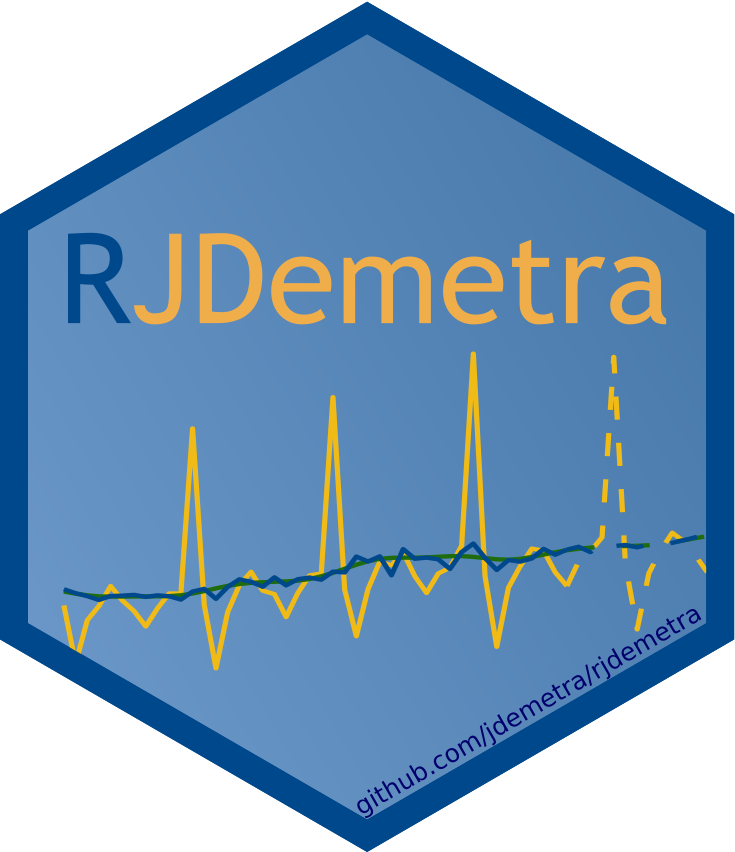
\includegraphics[width=4cm]{img/rjdemetra_logo.png}
\end{center}
\end{column}
\begin{column}{0.5\textwidth} 
\href{https://github.com/jdemetra/rjdemetra}{\faGithub{} jdemetra/rjdemetra}  

\href{https://twitter.com/JDemetraPlus}{\faTwitter{} @JdemetraPlus}

Other works and packages around JD+:  
\href{https://github.com/nbbrd}{\faGithub{} nbbrd}  
\end{column}
\end{columns}

\end{frame}

\end{document}
